% Options for packages loaded elsewhere
\PassOptionsToPackage{unicode}{hyperref}
\PassOptionsToPackage{hyphens}{url}
\PassOptionsToPackage{dvipsnames,svgnames,x11names}{xcolor}
%
\documentclass[
  letterpaper,
  DIV=11,
  numbers=noendperiod]{scrreprt}

\usepackage{amsmath,amssymb}
\usepackage{iftex}
\ifPDFTeX
  \usepackage[T1]{fontenc}
  \usepackage[utf8]{inputenc}
  \usepackage{textcomp} % provide euro and other symbols
\else % if luatex or xetex
  \usepackage{unicode-math}
  \defaultfontfeatures{Scale=MatchLowercase}
  \defaultfontfeatures[\rmfamily]{Ligatures=TeX,Scale=1}
\fi
\usepackage{lmodern}
\ifPDFTeX\else  
    % xetex/luatex font selection
\fi
% Use upquote if available, for straight quotes in verbatim environments
\IfFileExists{upquote.sty}{\usepackage{upquote}}{}
\IfFileExists{microtype.sty}{% use microtype if available
  \usepackage[]{microtype}
  \UseMicrotypeSet[protrusion]{basicmath} % disable protrusion for tt fonts
}{}
\makeatletter
\@ifundefined{KOMAClassName}{% if non-KOMA class
  \IfFileExists{parskip.sty}{%
    \usepackage{parskip}
  }{% else
    \setlength{\parindent}{0pt}
    \setlength{\parskip}{6pt plus 2pt minus 1pt}}
}{% if KOMA class
  \KOMAoptions{parskip=half}}
\makeatother
\usepackage{xcolor}
\setlength{\emergencystretch}{3em} % prevent overfull lines
\setcounter{secnumdepth}{5}
% Make \paragraph and \subparagraph free-standing
\makeatletter
\ifx\paragraph\undefined\else
  \let\oldparagraph\paragraph
  \renewcommand{\paragraph}{
    \@ifstar
      \xxxParagraphStar
      \xxxParagraphNoStar
  }
  \newcommand{\xxxParagraphStar}[1]{\oldparagraph*{#1}\mbox{}}
  \newcommand{\xxxParagraphNoStar}[1]{\oldparagraph{#1}\mbox{}}
\fi
\ifx\subparagraph\undefined\else
  \let\oldsubparagraph\subparagraph
  \renewcommand{\subparagraph}{
    \@ifstar
      \xxxSubParagraphStar
      \xxxSubParagraphNoStar
  }
  \newcommand{\xxxSubParagraphStar}[1]{\oldsubparagraph*{#1}\mbox{}}
  \newcommand{\xxxSubParagraphNoStar}[1]{\oldsubparagraph{#1}\mbox{}}
\fi
\makeatother

\usepackage{color}
\usepackage{fancyvrb}
\newcommand{\VerbBar}{|}
\newcommand{\VERB}{\Verb[commandchars=\\\{\}]}
\DefineVerbatimEnvironment{Highlighting}{Verbatim}{commandchars=\\\{\}}
% Add ',fontsize=\small' for more characters per line
\usepackage{framed}
\definecolor{shadecolor}{RGB}{241,243,245}
\newenvironment{Shaded}{\begin{snugshade}}{\end{snugshade}}
\newcommand{\AlertTok}[1]{\textcolor[rgb]{0.68,0.00,0.00}{#1}}
\newcommand{\AnnotationTok}[1]{\textcolor[rgb]{0.37,0.37,0.37}{#1}}
\newcommand{\AttributeTok}[1]{\textcolor[rgb]{0.40,0.45,0.13}{#1}}
\newcommand{\BaseNTok}[1]{\textcolor[rgb]{0.68,0.00,0.00}{#1}}
\newcommand{\BuiltInTok}[1]{\textcolor[rgb]{0.00,0.23,0.31}{#1}}
\newcommand{\CharTok}[1]{\textcolor[rgb]{0.13,0.47,0.30}{#1}}
\newcommand{\CommentTok}[1]{\textcolor[rgb]{0.37,0.37,0.37}{#1}}
\newcommand{\CommentVarTok}[1]{\textcolor[rgb]{0.37,0.37,0.37}{\textit{#1}}}
\newcommand{\ConstantTok}[1]{\textcolor[rgb]{0.56,0.35,0.01}{#1}}
\newcommand{\ControlFlowTok}[1]{\textcolor[rgb]{0.00,0.23,0.31}{\textbf{#1}}}
\newcommand{\DataTypeTok}[1]{\textcolor[rgb]{0.68,0.00,0.00}{#1}}
\newcommand{\DecValTok}[1]{\textcolor[rgb]{0.68,0.00,0.00}{#1}}
\newcommand{\DocumentationTok}[1]{\textcolor[rgb]{0.37,0.37,0.37}{\textit{#1}}}
\newcommand{\ErrorTok}[1]{\textcolor[rgb]{0.68,0.00,0.00}{#1}}
\newcommand{\ExtensionTok}[1]{\textcolor[rgb]{0.00,0.23,0.31}{#1}}
\newcommand{\FloatTok}[1]{\textcolor[rgb]{0.68,0.00,0.00}{#1}}
\newcommand{\FunctionTok}[1]{\textcolor[rgb]{0.28,0.35,0.67}{#1}}
\newcommand{\ImportTok}[1]{\textcolor[rgb]{0.00,0.46,0.62}{#1}}
\newcommand{\InformationTok}[1]{\textcolor[rgb]{0.37,0.37,0.37}{#1}}
\newcommand{\KeywordTok}[1]{\textcolor[rgb]{0.00,0.23,0.31}{\textbf{#1}}}
\newcommand{\NormalTok}[1]{\textcolor[rgb]{0.00,0.23,0.31}{#1}}
\newcommand{\OperatorTok}[1]{\textcolor[rgb]{0.37,0.37,0.37}{#1}}
\newcommand{\OtherTok}[1]{\textcolor[rgb]{0.00,0.23,0.31}{#1}}
\newcommand{\PreprocessorTok}[1]{\textcolor[rgb]{0.68,0.00,0.00}{#1}}
\newcommand{\RegionMarkerTok}[1]{\textcolor[rgb]{0.00,0.23,0.31}{#1}}
\newcommand{\SpecialCharTok}[1]{\textcolor[rgb]{0.37,0.37,0.37}{#1}}
\newcommand{\SpecialStringTok}[1]{\textcolor[rgb]{0.13,0.47,0.30}{#1}}
\newcommand{\StringTok}[1]{\textcolor[rgb]{0.13,0.47,0.30}{#1}}
\newcommand{\VariableTok}[1]{\textcolor[rgb]{0.07,0.07,0.07}{#1}}
\newcommand{\VerbatimStringTok}[1]{\textcolor[rgb]{0.13,0.47,0.30}{#1}}
\newcommand{\WarningTok}[1]{\textcolor[rgb]{0.37,0.37,0.37}{\textit{#1}}}

\providecommand{\tightlist}{%
  \setlength{\itemsep}{0pt}\setlength{\parskip}{0pt}}\usepackage{longtable,booktabs,array}
\usepackage{calc} % for calculating minipage widths
% Correct order of tables after \paragraph or \subparagraph
\usepackage{etoolbox}
\makeatletter
\patchcmd\longtable{\par}{\if@noskipsec\mbox{}\fi\par}{}{}
\makeatother
% Allow footnotes in longtable head/foot
\IfFileExists{footnotehyper.sty}{\usepackage{footnotehyper}}{\usepackage{footnote}}
\makesavenoteenv{longtable}
\usepackage{graphicx}
\makeatletter
\def\maxwidth{\ifdim\Gin@nat@width>\linewidth\linewidth\else\Gin@nat@width\fi}
\def\maxheight{\ifdim\Gin@nat@height>\textheight\textheight\else\Gin@nat@height\fi}
\makeatother
% Scale images if necessary, so that they will not overflow the page
% margins by default, and it is still possible to overwrite the defaults
% using explicit options in \includegraphics[width, height, ...]{}
\setkeys{Gin}{width=\maxwidth,height=\maxheight,keepaspectratio}
% Set default figure placement to htbp
\makeatletter
\def\fps@figure{htbp}
\makeatother
% definitions for citeproc citations
\NewDocumentCommand\citeproctext{}{}
\NewDocumentCommand\citeproc{mm}{%
  \begingroup\def\citeproctext{#2}\cite{#1}\endgroup}
\makeatletter
 % allow citations to break across lines
 \let\@cite@ofmt\@firstofone
 % avoid brackets around text for \cite:
 \def\@biblabel#1{}
 \def\@cite#1#2{{#1\if@tempswa , #2\fi}}
\makeatother
\newlength{\cslhangindent}
\setlength{\cslhangindent}{1.5em}
\newlength{\csllabelwidth}
\setlength{\csllabelwidth}{3em}
\newenvironment{CSLReferences}[2] % #1 hanging-indent, #2 entry-spacing
 {\begin{list}{}{%
  \setlength{\itemindent}{0pt}
  \setlength{\leftmargin}{0pt}
  \setlength{\parsep}{0pt}
  % turn on hanging indent if param 1 is 1
  \ifodd #1
   \setlength{\leftmargin}{\cslhangindent}
   \setlength{\itemindent}{-1\cslhangindent}
  \fi
  % set entry spacing
  \setlength{\itemsep}{#2\baselineskip}}}
 {\end{list}}
\usepackage{calc}
\newcommand{\CSLBlock}[1]{\hfill\break\parbox[t]{\linewidth}{\strut\ignorespaces#1\strut}}
\newcommand{\CSLLeftMargin}[1]{\parbox[t]{\csllabelwidth}{\strut#1\strut}}
\newcommand{\CSLRightInline}[1]{\parbox[t]{\linewidth - \csllabelwidth}{\strut#1\strut}}
\newcommand{\CSLIndent}[1]{\hspace{\cslhangindent}#1}

\KOMAoption{captions}{tableheading}
\makeatletter
\@ifpackageloaded{bookmark}{}{\usepackage{bookmark}}
\makeatother
\makeatletter
\@ifpackageloaded{caption}{}{\usepackage{caption}}
\AtBeginDocument{%
\ifdefined\contentsname
  \renewcommand*\contentsname{Table of contents}
\else
  \newcommand\contentsname{Table of contents}
\fi
\ifdefined\listfigurename
  \renewcommand*\listfigurename{List of Figures}
\else
  \newcommand\listfigurename{List of Figures}
\fi
\ifdefined\listtablename
  \renewcommand*\listtablename{List of Tables}
\else
  \newcommand\listtablename{List of Tables}
\fi
\ifdefined\figurename
  \renewcommand*\figurename{Figure}
\else
  \newcommand\figurename{Figure}
\fi
\ifdefined\tablename
  \renewcommand*\tablename{Table}
\else
  \newcommand\tablename{Table}
\fi
}
\@ifpackageloaded{float}{}{\usepackage{float}}
\floatstyle{ruled}
\@ifundefined{c@chapter}{\newfloat{codelisting}{h}{lop}}{\newfloat{codelisting}{h}{lop}[chapter]}
\floatname{codelisting}{Listing}
\newcommand*\listoflistings{\listof{codelisting}{List of Listings}}
\makeatother
\makeatletter
\makeatother
\makeatletter
\@ifpackageloaded{caption}{}{\usepackage{caption}}
\@ifpackageloaded{subcaption}{}{\usepackage{subcaption}}
\makeatother

\ifLuaTeX
  \usepackage{selnolig}  % disable illegal ligatures
\fi
\usepackage{bookmark}

\IfFileExists{xurl.sty}{\usepackage{xurl}}{} % add URL line breaks if available
\urlstyle{same} % disable monospaced font for URLs
\hypersetup{
  pdftitle={Modelovanie ekonomických procesov},
  pdfauthor={Darth Vader},
  colorlinks=true,
  linkcolor={blue},
  filecolor={Maroon},
  citecolor={Blue},
  urlcolor={Blue},
  pdfcreator={LaTeX via pandoc}}


\title{Modelovanie ekonomických procesov}
\author{Darth Vader}
\date{2025-03-23}

\begin{document}
\maketitle

\renewcommand*\contentsname{Table of contents}
{
\hypersetup{linkcolor=}
\setcounter{tocdepth}{2}
\tableofcontents
}

\bookmarksetup{startatroot}

\chapter*{Preface}\label{preface}
\addcontentsline{toc}{chapter}{Preface}

\markboth{Preface}{Preface}

Modelovanie Ekonomických procesov

\bookmarksetup{startatroot}

\chapter*{Úvod}\label{uxfavod}
\addcontentsline{toc}{chapter}{Úvod}

\markboth{Úvod}{Úvod}

\part{Úvod do časových radov}

\chapter{Úvod do časových
radov}\label{uxfavod-do-ux10dasovuxfdch-radov-1}

Použijeme dáta o požičiavaní bicyklov. Dátový súbor je dostupný na
href=``https://archive.ics.uci.edu/ml/datasets/Bike+Sharing+Dataset''\textgreater{}
adrese kde sú vysvetlené aj premenné. Budeme používať dáta o dennom
požičiavaní bicyklov. Závislá premenná bude ``cnt'', ktorá v sebe zahrňa
celkový počet bicyklov požičaných za deň pre obe skupiny ľudí aj
registrovaných aj príležitostných.

Údaje môžete načítať do R pomocou funkcie read.csv(), ktorá predpokladá,
že vaše údaje sú po sebe idúce časové body v jednoduchom textovom súbore
s jedným stĺpcom. Keď načítate údaje časových radov do R, ďalším krokom
je uloženie údajov do objektu časových radov v R, aby ste mohli použiť
mnohé funkcie R na analýzu údajov časových radov. Na uloženie údajov do
objektu časového radu používame funkciu ts() v R. Napríklad na uloženie
údajov do premennej `bike' ako objektu časového radu v R napíšeme:

\begin{Shaded}
\begin{Highlighting}[]
\FunctionTok{library}\NormalTok{(tseries)}
\end{Highlighting}
\end{Shaded}

\begin{verbatim}
Registered S3 method overwritten by 'quantmod':
  method            from
  as.zoo.data.frame zoo 
\end{verbatim}

\begin{Shaded}
\begin{Highlighting}[]
\FunctionTok{library}\NormalTok{(TTR)}
\NormalTok{bike }\OtherTok{\textless{}{-}} \FunctionTok{read.csv}\NormalTok{(}\StringTok{"dayBike.csv"}\NormalTok{, }\AttributeTok{header=}\ConstantTok{TRUE}\NormalTok{, }\AttributeTok{stringsAsFactors=}\ConstantTok{FALSE}\NormalTok{)}
\FunctionTok{str}\NormalTok{(bike)}
\end{Highlighting}
\end{Shaded}

\begin{verbatim}
'data.frame':   731 obs. of  16 variables:
 $ instant   : int  1 2 3 4 5 6 7 8 9 10 ...
 $ dteday    : chr  "2011-01-01" "2011-01-02" "2011-01-03" "2011-01-04" ...
 $ season    : int  1 1 1 1 1 1 1 1 1 1 ...
 $ yr        : int  0 0 0 0 0 0 0 0 0 0 ...
 $ mnth      : int  1 1 1 1 1 1 1 1 1 1 ...
 $ holiday   : int  0 0 0 0 0 0 0 0 0 0 ...
 $ weekday   : int  6 0 1 2 3 4 5 6 0 1 ...
 $ workingday: int  0 0 1 1 1 1 1 0 0 1 ...
 $ weathersit: int  2 2 1 1 1 1 2 2 1 1 ...
 $ temp      : num  0.344 0.363 0.196 0.2 0.227 ...
 $ atemp     : num  0.364 0.354 0.189 0.212 0.229 ...
 $ hum       : num  0.806 0.696 0.437 0.59 0.437 ...
 $ windspeed : num  0.16 0.249 0.248 0.16 0.187 ...
 $ casual    : int  331 131 120 108 82 88 148 68 54 41 ...
 $ registered: int  654 670 1229 1454 1518 1518 1362 891 768 1280 ...
 $ cnt       : int  985 801 1349 1562 1600 1606 1510 959 822 1321 ...
\end{verbatim}

\begin{Shaded}
\begin{Highlighting}[]
\FunctionTok{head}\NormalTok{(bike,}\AttributeTok{n=}\DecValTok{10}\NormalTok{)}
\end{Highlighting}
\end{Shaded}

\begin{verbatim}
   instant     dteday season yr mnth holiday weekday workingday weathersit
1        1 2011-01-01      1  0    1       0       6          0          2
2        2 2011-01-02      1  0    1       0       0          0          2
3        3 2011-01-03      1  0    1       0       1          1          1
4        4 2011-01-04      1  0    1       0       2          1          1
5        5 2011-01-05      1  0    1       0       3          1          1
6        6 2011-01-06      1  0    1       0       4          1          1
7        7 2011-01-07      1  0    1       0       5          1          2
8        8 2011-01-08      1  0    1       0       6          0          2
9        9 2011-01-09      1  0    1       0       0          0          1
10      10 2011-01-10      1  0    1       0       1          1          1
       temp    atemp      hum windspeed casual registered  cnt
1  0.344167 0.363625 0.805833 0.1604460    331        654  985
2  0.363478 0.353739 0.696087 0.2485390    131        670  801
3  0.196364 0.189405 0.437273 0.2483090    120       1229 1349
4  0.200000 0.212122 0.590435 0.1602960    108       1454 1562
5  0.226957 0.229270 0.436957 0.1869000     82       1518 1600
6  0.204348 0.233209 0.518261 0.0895652     88       1518 1606
7  0.196522 0.208839 0.498696 0.1687260    148       1362 1510
8  0.165000 0.162254 0.535833 0.2668040     68        891  959
9  0.138333 0.116175 0.434167 0.3619500     54        768  822
10 0.150833 0.150888 0.482917 0.2232670     41       1280 1321
\end{verbatim}

\begin{Shaded}
\begin{Highlighting}[]
\NormalTok{bike}\SpecialCharTok{$}\NormalTok{Date  }\OtherTok{\textless{}{-}} \FunctionTok{as.Date}\NormalTok{(bike}\SpecialCharTok{$}\NormalTok{dteday)}
\NormalTok{countBike }\OtherTok{\textless{}{-}} \FunctionTok{ts}\NormalTok{(bike[, }\FunctionTok{c}\NormalTok{(}\StringTok{\textquotesingle{}cnt\textquotesingle{}}\NormalTok{)])}
\end{Highlighting}
\end{Shaded}

Prvá vec, ktorú budete chcieť urobiť pri analýze údajov časových radov,
bude načítať ich do R a vykresliť časový rad.

\begin{Shaded}
\begin{Highlighting}[]
\FunctionTok{plot.ts}\NormalTok{(countBike)}
\end{Highlighting}
\end{Shaded}

\includegraphics{prednaska1_UvodCasoveRady_files/figure-pdf/unnamed-chunk-2-1.pdf}

Z časového grafu vidíme, že tento časový rad by sa dal pravdepodobne
opísať pomocou aditívneho modelu, pretože náhodné výkyvy v údajoch majú
v čase zhruba konštantnú veľkosť

Niekedy sa množina údajov časových radov, ktorú máte, mohla zhromažďovať
v pravidelných intervaloch kratších ako jeden rok, napríklad mesačne
alebo štvrťročne. V tomto prípade môžete pomocou parametra „frekvencia``
vo funkcii ts() určiť, koľkokrát boli údaje za rok zhromaždené. Pre
mesačné údaje časových radov nastavíte frekvenciu = 12, zatiaľ čo pre
štvrťročné údaje časových radov nastavíte frekvenciu = 4.

Príkladom sezónnych údajov je súbor údajov o počte pôrodov za mesiac v
meste New York od januára 1946 do decembra 1959. Tieto údaje sú dostupné
v súbore ``NewYorkBirths.csv'' Údaje môžeme načítať do R a uložiť ich
ako objekt časovej rady zadaním:

\begin{Shaded}
\begin{Highlighting}[]
\NormalTok{births }\OtherTok{\textless{}{-}} \FunctionTok{read.csv}\NormalTok{(}\StringTok{"NewYorkBirths.csv"}\NormalTok{, }\AttributeTok{header=}\ConstantTok{TRUE}\NormalTok{, }\AttributeTok{stringsAsFactors=}\ConstantTok{FALSE}\NormalTok{)}
\FunctionTok{head}\NormalTok{(births)}
\end{Highlighting}
\end{Shaded}

\begin{verbatim}
  X      x
1 1 26.663
2 2 23.598
3 3 26.931
4 4 24.740
5 5 25.806
6 6 24.364
\end{verbatim}

\begin{Shaded}
\begin{Highlighting}[]
\NormalTok{births }\OtherTok{\textless{}{-}}\NormalTok{ births[,}\FunctionTok{c}\NormalTok{(}\StringTok{"x"}\NormalTok{)]}
\NormalTok{birthsts }\OtherTok{\textless{}{-}} \FunctionTok{ts}\NormalTok{(births, }\AttributeTok{frequency=}\DecValTok{12}\NormalTok{, }\AttributeTok{start=}\FunctionTok{c}\NormalTok{(}\DecValTok{1946}\NormalTok{,}\DecValTok{1}\NormalTok{))}
\FunctionTok{head}\NormalTok{(birthsts)}
\end{Highlighting}
\end{Shaded}

\begin{verbatim}
[1] 26.663 23.598 26.931 24.740 25.806 24.364
\end{verbatim}

\begin{Shaded}
\begin{Highlighting}[]
\FunctionTok{plot.ts}\NormalTok{(birthsts)}
\end{Highlighting}
\end{Shaded}

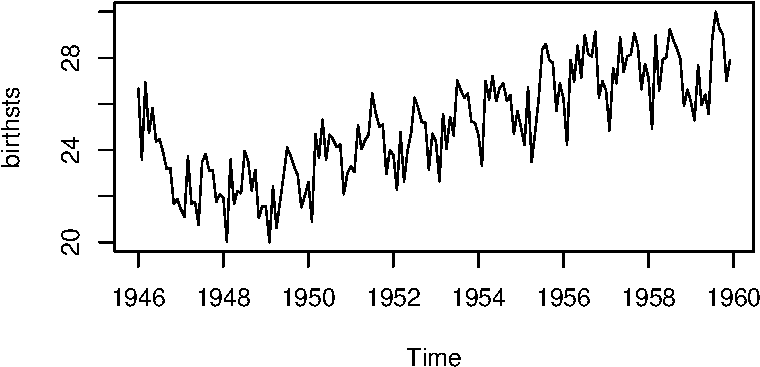
\includegraphics{prednaska1_UvodCasoveRady_files/figure-pdf/unnamed-chunk-3-1.pdf}

Z tohto časového radu vidíme, že sa zdá, že v počte pôrodov za mesiac
existujú sezónne variácie: každé leto je vrchol a každú zimu je
najnižší. Opäť sa zdá, že tento časový rad by sa dal pravdepodobne
opísať pomocou aditívneho modelu, pretože sezónne výkyvy sú v priebehu
času zhruba konštantné a nezdá sa, že by záviseli od úrovne časového
radu a náhodné výkyvy sa tiež zdajú byť v priebehu času zhruba
konštantnej veľkosti.

\section{Dekompozícia časových
radov}\label{dekompozuxedcia-ux10dasovuxfdch-radov}

Rozloženie časového radu znamená jeho rozdelenie na jednotlivé zložky,
ktorými sú zvyčajne trendová zložka a nepravidelná zložka, a ak ide o
sezónny časový rad, sezónna zložka.

Nesezónny časový rad pozostáva z trendovej zložky a nepravidelnej
zložky. Dekompozícia časového radu zahŕňa snahu rozdeliť časový rad na
tieto zložky, čiže odhadnúť trendovú zložku a nepravidelnú zložku.

\subsection{Trend zložka}\label{trend-zloux17eka}

Na odhadnutie trendovej zložky nesezónneho časového radu, ktorý možno
opísať pomocou aditívneho modelu, sa bežne používa metóda vyrovnávania
(vyhladzovania), ako je napríklad výpočet jednoduchého kĺzavého priemeru
časového radu.

Funkciu SMA() (Simple Moving Average) v balíku „TTR``
(https://bookdown.org/kochiuyu/technical-analysis-with-r-second-edition/technical-indicators.html)
R možno použiť na vyhladenie údajov časových radov pomocou jednoduchého
kĺzavého priemeru. Ak chcete použiť túto funkciu, musíme najprv
nainštalovať balík „TTR`` R (návod na inštaláciu balíka R nájdete v
časti Ako nainštalovať balík R ).

Potom môžete použiť funkciu „SMA()`` na vyhladenie údajov časových
radov. Ak chcete použiť funkciu SMA(), musíte zadať poradie (rozpätie)
jednoduchého kĺzavého priemeru pomocou parametra „n``. Napríklad na
výpočet jednoduchého kĺzavého priemeru rádu 5 nastavíme n=5 vo funkcii
SMA().

Napríklad, ako je uvedené vyššie, časový rad počtu požičaných bicyklov
za deň sa javia ako nesezónne a možno ich pravdepodobne opísať pomocou
aditívneho modelu, pretože náhodné výkyvy v údajoch sú zhruba
konštantné. Môžeme sa teda pokúsiť odhadnúť trendovú zložku tohto
časového radu vyhladením pomocou jednoduchého kĺzavého priemeru. Na
vyhladenie časového radu pomocou jednoduchého kĺzavého priemeru rádu 30
(mesiac) a vykreslenie údajov vyhladeného časového radu napíšeme:

\begin{Shaded}
\begin{Highlighting}[]
\NormalTok{countBikeSMA30 }\OtherTok{\textless{}{-}} \FunctionTok{SMA}\NormalTok{(countBike,}\AttributeTok{n=}\DecValTok{30}\NormalTok{)}
\FunctionTok{plot.ts}\NormalTok{(countBikeSMA30,}\AttributeTok{col =} \StringTok{"blue"}\NormalTok{)}
\FunctionTok{lines}\NormalTok{(countBike)}
\end{Highlighting}
\end{Shaded}

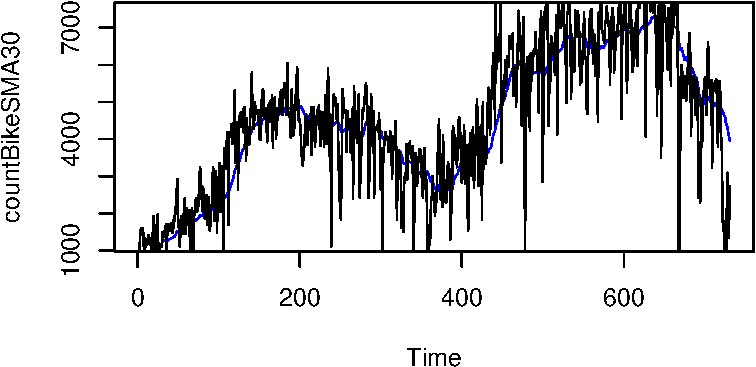
\includegraphics{prednaska1_UvodCasoveRady_files/figure-pdf/unnamed-chunk-4-1.pdf}

Údaje vyhladené jednoduchým kĺzavým priemerom rádu 30 poskytujú jasnejší
obraz trendovej zložky a môžeme vidieť, že časové rady počtu požičaných
bicyklov za deň stúpal postupne až na hodnoty okolo 7000 a začal kolísať
okolo 6000 s náhodnými poklesmi pod 5000.

\subsection{Sezónna zložka}\label{sezuxf3nna-zloux17eka}

Sezónny časový rad pozostáva z trendovej zložky, sezónnej zložky a
nepravidelnej zložky. Rozloženie časového radu znamená rozdelenie
časového radu na tieto tri zložky: teda odhad týchto troch zložiek.

Na odhadnutie trendovej zložky a sezónnej zložky sezónneho časového
radu, ktoré možno opísať pomocou aditívneho modelu, môžeme použiť
funkciu „decompose()`` v R. Táto funkcia odhaduje trendové, sezónne a
nepravidelné zložky časového radu ktoré možno opísať pomocou aditívneho
modelu.

Funkcia „decompose()`` vráti ako výsledok objekt zoznamu, kde sú odhady
sezónneho komponentu, komponentu trendu a nepravidelného komponentu
uložené v pomenovaných prvkoch týchto objektov zoznamu, ktoré sa
nazývajú „sezónne``, „trend`` a „náhodné``. ``.

Napríklad, ako je uvedené vyššie, časový rad počtu pôrodov za mesiac v
meste New York je sezónny s vrcholom každé leto a minimom každú zimu a
možno ho pravdepodobne opísať pomocou aditívneho modelu, pretože sezónne
a náhodné výkyvy sa zdajú byť mať v priebehu času zhruba konštantnú
veľkosť. Na odhad trendových, sezónnych a nepravidelných zložiek tohto
časového radu napíšeme:

\begin{Shaded}
\begin{Highlighting}[]
\NormalTok{birthstscomponents }\OtherTok{\textless{}{-}} \FunctionTok{decompose}\NormalTok{(birthsts)}
\end{Highlighting}
\end{Shaded}

Odhadované hodnoty sezónneho, trendového a nepravidelného komponentu sú
teraz uložené v premenných komponenty
birthstscomponents\(seasonal, birthstscomponents\)trend and
birthstscomponents\$random. Napríklad odhadované hodnoty sezónnej zložky
môžeme vidieť zadaním:

\begin{Shaded}
\begin{Highlighting}[]
\CommentTok{\# birthstscomponents$seasonal}
\end{Highlighting}
\end{Shaded}

Odhadované sezónne faktory (birthstscomponents\$seasonal) sú uvedené pre
mesiace január až december a sú rovnaké pre každý rok. Najväčší sezónny
faktor je za júl (približne 1,46) a najnižší za február (približne
-2,08), čo naznačuje, že sa zdá, že každý rok je vrchol pôrodov v júli a
najnižší počet narodených vo februári.

\begin{Shaded}
\begin{Highlighting}[]
\CommentTok{\# birthstscomponents$trend}
\CommentTok{\# birthstscomponents$random}
\end{Highlighting}
\end{Shaded}

Odhadovaný trend, sezónne a nepravidelné zložky časového radu môžeme
vykresliť pomocou funkcie „plot()``, napríklad:

\begin{Shaded}
\begin{Highlighting}[]
\FunctionTok{plot}\NormalTok{(birthstscomponents)}
\end{Highlighting}
\end{Shaded}

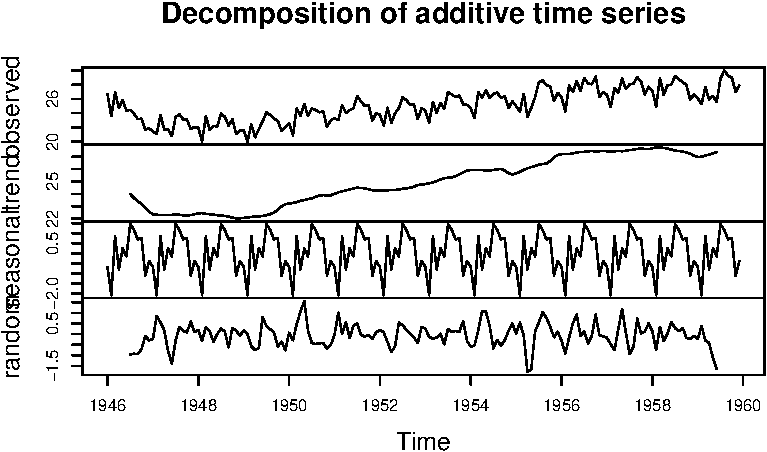
\includegraphics{prednaska1_UvodCasoveRady_files/figure-pdf/unnamed-chunk-8-1.pdf}

Uvedený dekompozičný graf zobrazuje pôvodný časový rad mesačných pôrodov
v NY, odhadovanú trendovú zložku (druhá zhora), odhadovanú sezónnu
zložku (tretia zhora) a odhadovanú nepravidelnú zložku (dole). Vidíme,
že zložka odhadovaného trendu vykazuje malý pokles z približne 24 tisíc
v roku 1947 na približne 22 tisíc v roku 1948, po ktorom nasleduje
stabilný nárast na približne 27 tisíc v roku 1959.

Ak máte sezónny časový rad, ktorý možno opísať pomocou aditívneho
modelu, môžete ho sezónne upraviť odhadom sezónnej zložky a odpočítaním
odhadovanej sezónnej zložky od pôvodného časového radu. Môžeme to urobiť
pomocou odhadu sezónnej zložky vypočítanej funkciou „decompose()``.

Napríklad, aby sme sezónne upravili časový rad počtu pôrodov za mesiac v
New Yorku, môžeme odhadnúť sezónny komponent pomocou „decompose()`` a
potom odpočítať sezónny komponent od pôvodného časového radu:

\begin{Shaded}
\begin{Highlighting}[]
\NormalTok{birthstsseasonallyadjusted }\OtherTok{\textless{}{-}}\NormalTok{ birthsts }\SpecialCharTok{{-}} \FunctionTok{head}\NormalTok{(birthstscomponents}\SpecialCharTok{$}\NormalTok{seasonal)}
\end{Highlighting}
\end{Shaded}

Potom môžeme vykresliť sezónne upravené časové rady pomocou funkcie
„plot()`` zadaním:

\begin{Shaded}
\begin{Highlighting}[]
\FunctionTok{plot}\NormalTok{(birthstsseasonallyadjusted)}
\end{Highlighting}
\end{Shaded}

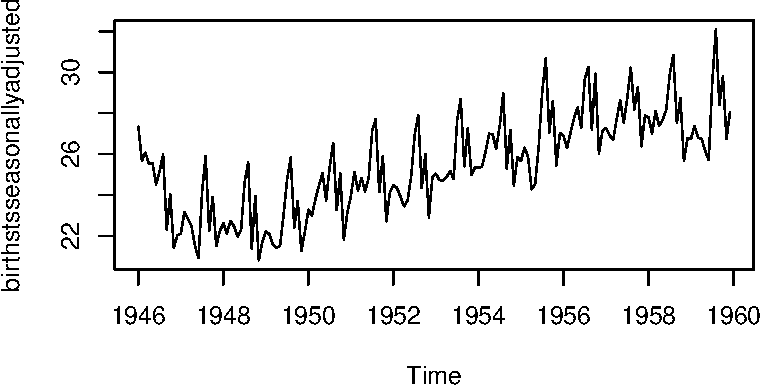
\includegraphics{prednaska1_UvodCasoveRady_files/figure-pdf/unnamed-chunk-10-1.pdf}

Môžete vidieť, že sezónna variácia bola odstránená zo sezónne očisteného
časového radu. Sezónne očistený časový rad obsahuje už len trendovú
zložku a nepravidelnú zložku.

\part{Holt Winters exponenciálne vyrovnávanie dát}

\chapter{Dáta o požičiavaní
bicyklov}\label{duxe1ta-o-poux17eiux10diavanuxed-bicyklov}

Údaje môžete načítať do R pomocou funkcie read.csv(), ktorá predpokladá,
že vaše údaje sú po sebe idúce časové body v jednoduchom textovom súbore
s jedným stĺpcom. Keď načítate údaje časových radov do R, ďalším krokom
je uloženie údajov do objektu časových radov v R, aby ste mohli použiť
mnohé funkcie R na analýzu údajov časových radov. Na uloženie údajov do
objektu časového radu používame funkciu ts() v R. Napríklad na uloženie
údajov do premennej `bike' ako objektu časového radu v R napíšeme:

\begin{Shaded}
\begin{Highlighting}[]
\FunctionTok{library}\NormalTok{(tseries)}
\end{Highlighting}
\end{Shaded}

\begin{verbatim}
Registered S3 method overwritten by 'quantmod':
  method            from
  as.zoo.data.frame zoo 
\end{verbatim}

\begin{Shaded}
\begin{Highlighting}[]
\FunctionTok{library}\NormalTok{(TTR)}
\NormalTok{bike }\OtherTok{\textless{}{-}} \FunctionTok{read.csv}\NormalTok{(}\StringTok{"dayBike.csv"}\NormalTok{, }\AttributeTok{header=}\ConstantTok{TRUE}\NormalTok{, }\AttributeTok{stringsAsFactors=}\ConstantTok{FALSE}\NormalTok{)}
\FunctionTok{str}\NormalTok{(bike)}
\end{Highlighting}
\end{Shaded}

\begin{verbatim}
'data.frame':   731 obs. of  16 variables:
 $ instant   : int  1 2 3 4 5 6 7 8 9 10 ...
 $ dteday    : chr  "2011-01-01" "2011-01-02" "2011-01-03" "2011-01-04" ...
 $ season    : int  1 1 1 1 1 1 1 1 1 1 ...
 $ yr        : int  0 0 0 0 0 0 0 0 0 0 ...
 $ mnth      : int  1 1 1 1 1 1 1 1 1 1 ...
 $ holiday   : int  0 0 0 0 0 0 0 0 0 0 ...
 $ weekday   : int  6 0 1 2 3 4 5 6 0 1 ...
 $ workingday: int  0 0 1 1 1 1 1 0 0 1 ...
 $ weathersit: int  2 2 1 1 1 1 2 2 1 1 ...
 $ temp      : num  0.344 0.363 0.196 0.2 0.227 ...
 $ atemp     : num  0.364 0.354 0.189 0.212 0.229 ...
 $ hum       : num  0.806 0.696 0.437 0.59 0.437 ...
 $ windspeed : num  0.16 0.249 0.248 0.16 0.187 ...
 $ casual    : int  331 131 120 108 82 88 148 68 54 41 ...
 $ registered: int  654 670 1229 1454 1518 1518 1362 891 768 1280 ...
 $ cnt       : int  985 801 1349 1562 1600 1606 1510 959 822 1321 ...
\end{verbatim}

\begin{Shaded}
\begin{Highlighting}[]
\FunctionTok{head}\NormalTok{(bike,}\AttributeTok{n=}\DecValTok{10}\NormalTok{)}
\end{Highlighting}
\end{Shaded}

\begin{verbatim}
   instant     dteday season yr mnth holiday weekday workingday weathersit
1        1 2011-01-01      1  0    1       0       6          0          2
2        2 2011-01-02      1  0    1       0       0          0          2
3        3 2011-01-03      1  0    1       0       1          1          1
4        4 2011-01-04      1  0    1       0       2          1          1
5        5 2011-01-05      1  0    1       0       3          1          1
6        6 2011-01-06      1  0    1       0       4          1          1
7        7 2011-01-07      1  0    1       0       5          1          2
8        8 2011-01-08      1  0    1       0       6          0          2
9        9 2011-01-09      1  0    1       0       0          0          1
10      10 2011-01-10      1  0    1       0       1          1          1
       temp    atemp      hum windspeed casual registered  cnt
1  0.344167 0.363625 0.805833 0.1604460    331        654  985
2  0.363478 0.353739 0.696087 0.2485390    131        670  801
3  0.196364 0.189405 0.437273 0.2483090    120       1229 1349
4  0.200000 0.212122 0.590435 0.1602960    108       1454 1562
5  0.226957 0.229270 0.436957 0.1869000     82       1518 1600
6  0.204348 0.233209 0.518261 0.0895652     88       1518 1606
7  0.196522 0.208839 0.498696 0.1687260    148       1362 1510
8  0.165000 0.162254 0.535833 0.2668040     68        891  959
9  0.138333 0.116175 0.434167 0.3619500     54        768  822
10 0.150833 0.150888 0.482917 0.2232670     41       1280 1321
\end{verbatim}

\begin{Shaded}
\begin{Highlighting}[]
\NormalTok{bike}\SpecialCharTok{$}\NormalTok{Date  }\OtherTok{\textless{}{-}} \FunctionTok{as.Date}\NormalTok{(bike}\SpecialCharTok{$}\NormalTok{dteday)}
\NormalTok{countBike }\OtherTok{\textless{}{-}} \FunctionTok{ts}\NormalTok{(bike[, }\FunctionTok{c}\NormalTok{(}\StringTok{\textquotesingle{}cnt\textquotesingle{}}\NormalTok{)])}
\end{Highlighting}
\end{Shaded}

Prvá vec, ktorú budete chcieť urobiť pri analýze údajov časových radov,
bude načítať ich do R a vykresliť časový rad.

\begin{Shaded}
\begin{Highlighting}[]
\FunctionTok{plot.ts}\NormalTok{(countBike)}
\end{Highlighting}
\end{Shaded}

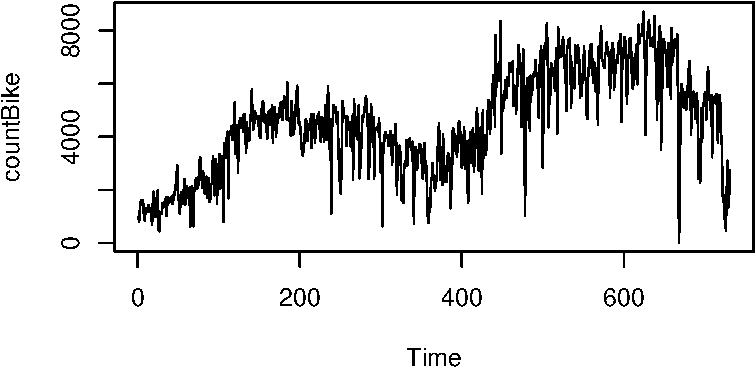
\includegraphics{prednaska2_HoltWinters_files/figure-pdf/unnamed-chunk-2-1.pdf}

\section{Jednoduché exponenciálne
vyrovnávanie}\label{jednoduchuxe9-exponenciuxe1lne-vyrovnuxe1vanie}

Ak máte časový rad, ktorý možno opísať pomocou aditívneho modelu s
konštantnou úrovňou a bez sezónnosti, môžete použiť jednoduché
exponenciálne vyhladzovanie na vytváranie krátkodobých predpovedí.

Jednoduchá metóda exponenciálneho vyhladzovania poskytuje spôsob odhadu
úrovne v aktuálnom časovom bode. Vyhladzovanie je riadené parametrom
alfa; pre odhad úrovne v aktuálnom časovom bode. hodnota alfa; leží
medzi 0 a 1. Hodnoty alfa, ktoré sú blízke 0, znamenajú, že pri
predpovediach budúcich hodnôt sa prikladá malá váha najnovším
pozorovaniam.

Na vytváranie predpovedí pomocou jednoduchého exponenciálneho
vyhladzovania v jazyku R môžeme použiť jednoduchý prediktívny model
exponenciálneho vyhladzovania pomocou funkcie „HoltWinters()`` v jazyku
R. Ak chcete použiť HoltWinters() na jednoduché exponenciálne
vyhladzovanie, musíme nastaviť parametre beta=FALSE a gamma=FALSE vo
funkcii HoltWinters() (parametre beta a gama sa používajú na Holtovo
exponenciálne vyhladzovanie alebo Holt-Wintersovo exponenciálne
vyhladzovanie, ako je popísané nižšie). Alfa je ``základná hodnota''.
Vyššie alfa prikladá väčšiu váhu najnovším pozorovaniam. Beta je
``trendová hodnota''. Vyššia beta znamená, že sklon trendu je viac
závislý od posledných sklonov trendu. Gama je ``sezónna zložka''. Vyššia
gama dáva väčšiu váhu najnovším sezónnym cyklom.

Funkcia HoltWinters() vracia premennú zoznamu, ktorá obsahuje niekoľko
pomenovaných prvkov.

Napríklad, ak chcete použiť jednoduché exponenciálne vyhladzovanie na
vytváranie predpovedí pre časový rad počtu požičaných bicyklov za deň,
napíšeme:

\begin{Shaded}
\begin{Highlighting}[]
\NormalTok{countBikeHW }\OtherTok{\textless{}{-}} \FunctionTok{HoltWinters}\NormalTok{(countBike, }\AttributeTok{beta=}\ConstantTok{FALSE}\NormalTok{, }\AttributeTok{gamma=}\ConstantTok{FALSE}\NormalTok{)}
\end{Highlighting}
\end{Shaded}

Výstup HoltWinters() nám hovorí, že odhadovaná hodnota parametra alfa je
približne 0.28. To je celkom ďalje od nuly, čo nám hovorí, že predpovede
sú založené na nedávnych pozorovaniach.

Vo vyššie uvedenom príklade sme uložili výstup funkcie HoltWinters() do
premennej zoznamu „countBikeHW``. Prognózy vytvorené HoltWinters() sú
uložené v pomenovanom objekte tejto premennej listu pod názvom
„fitted``, takže ich hodnoty môžeme získať zadaním:

\begin{Shaded}
\begin{Highlighting}[]
\FunctionTok{head}\NormalTok{(countBikeHW}\SpecialCharTok{$}\NormalTok{fitted)}
\end{Highlighting}
\end{Shaded}

\begin{verbatim}
         xhat    level
[1,]  985.000  985.000
[2,]  932.748  932.748
[3,] 1050.954 1050.954
[4,] 1196.080 1196.080
[5,] 1310.785 1310.785
[6,] 1394.619 1394.619
\end{verbatim}

Pôvodný časový rad môžeme vykresliť oproti expoeneciálnemu
vyrovnávanémuu radu zadaním:

\begin{Shaded}
\begin{Highlighting}[]
\FunctionTok{plot}\NormalTok{(countBikeHW)}
\FunctionTok{lines}\NormalTok{(countBike)}
\end{Highlighting}
\end{Shaded}

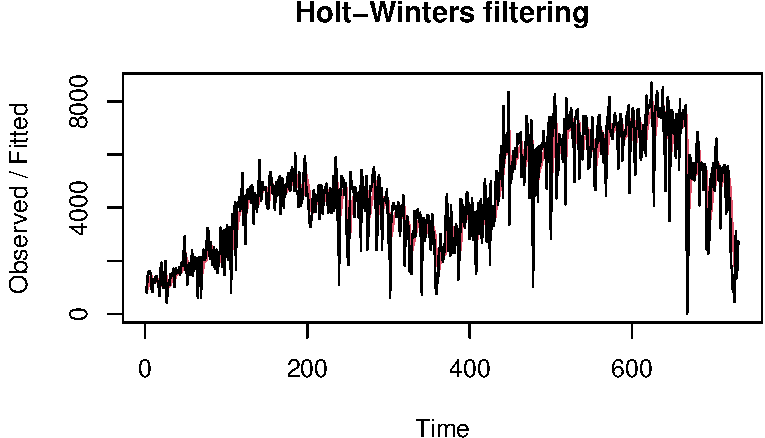
\includegraphics{prednaska2_HoltWinters_files/figure-pdf/unnamed-chunk-5-1.pdf}

\begin{Shaded}
\begin{Highlighting}[]
\NormalTok{countBikeHW}\SpecialCharTok{$}\NormalTok{SSE}
\end{Highlighting}
\end{Shaded}

\begin{verbatim}
[1] 680114835
\end{verbatim}

Graf zobrazuje pôvodný časový rad čiernou farbou a prognózy ako červenou
čiaru. Časový rad predpovedí je oveľa plynulejší ako časový rad
pôvodných údajov.

Ako mieru presnosti prognóz môžeme použiť súčet štvorcov chýb pre chyby
prognóz vo vzorke, t. j. chyby prognóz za časové obdobie, ktoré pokrýva
náš pôvodný časový rad. Suma štvorcov chýb je uložená v pomenovanom
prvku premennej zoznamu ``countBikeHW'' s názvom ``SSE'', takže jej
hodnotu môžeme získať zadaním ``countBikeHW\$SSE''. Súčet štvorcov chýb
je dosť vysoký.

\section{Holt Winters
prognózovanie}\label{holt-winters-prognuxf3zovanie}

Pri jednoduchom exponenciálnom vyhladzovaní je bežné použiť prvú hodnotu
v časovom rade ako počiatočnú hodnotu pre úroveň. Napríklad v časovom
rade pre požičané bicykle je prvá dňová hodnota 985 sledovaného
dvojročného obdobia. Počiatočnú hodnotu pre úroveň môžete určiť vo
funkcii HoltWinters() pomocou parametra ``l.start''. Ak chceme napríklad
vytvoriť predpoveď s počiatočnou hodnotou hladiny nastavenou na 985,
zadáme:

\begin{Shaded}
\begin{Highlighting}[]
\FunctionTok{HoltWinters}\NormalTok{(countBike, }\AttributeTok{beta=}\ConstantTok{FALSE}\NormalTok{, }\AttributeTok{gamma=}\ConstantTok{FALSE}\NormalTok{,}\AttributeTok{l.start=}\DecValTok{985}\NormalTok{)}
\end{Highlighting}
\end{Shaded}

\begin{verbatim}
Holt-Winters exponential smoothing without trend and without seasonal component.

Call:
HoltWinters(x = countBike, beta = FALSE, gamma = FALSE, l.start = 985)

Smoothing parameters:
 alpha: 0.2839781
 beta : FALSE
 gamma: FALSE

Coefficients:
      [,1]
a 2121.331
\end{verbatim}

Ako bolo vysvetlené vyššie, v predvolenom nastavení HoltWinters() sa
predpovede vytvárajú len pre časové obdobie, ktoré pokrývajú pôvodné
údaje, čo je v prípade časového radu pre požičané bicykle obdobie dvoch
seldovaných rokov. Predpovede pre ďalšie časové body môžeme vytvoriť
pomocou funkcie ``forecast.HoltWinters()'' v balíku R ``forecast''. Ak
chceme použiť funkciu forecast.HoltWinters(), musíme si najprv
nainštalovať balík R ``forecast''.

Pri použití funkcie forecast.HoltWinters() jej ako prvý argument (vstup)
odovzdáte predikčný model, ktorý ste už zostavili pomocou funkcie
HoltWinters(). Napríklad v prípade časového radu pre požičané bicykle
sme predikčný model vytvorený pomocou funkcie HoltWinters() uložili do
premennej ``countBikeHW''. Pomocou parametra ``h'' vo funkcii
forecast.HoltWinters() určíte, pre koľko ďalších časových bodov chcete
vytvoriť prognózy. Napríklad, ak chceme vytvoriť predpoveď požičané
bicykle na ďalšie dni (ďalších 7 dní) pomocou funkcie
forecast.HoltWinters(), zadáme:

\begin{Shaded}
\begin{Highlighting}[]
\NormalTok{countBikeHWforecast }\OtherTok{\textless{}{-}}\NormalTok{ forecast}\SpecialCharTok{:::}\FunctionTok{forecast.HoltWinters}\NormalTok{(countBikeHW, }\AttributeTok{h=}\DecValTok{7}\NormalTok{)}
\NormalTok{countBikeHWforecast}
\end{Highlighting}
\end{Shaded}

\begin{verbatim}
    Point Forecast    Lo 80    Hi 80      Lo 95    Hi 95
732       2121.331 883.5143 3359.148  228.25360 4014.409
733       2121.331 834.5710 3408.092  153.40116 4089.262
734       2121.331 787.4222 3455.240   81.29333 4161.369
735       2121.331 741.8840 3500.779   11.64867 4231.014
736       2121.331 697.8018 3544.861  -55.76922 4298.432
737       2121.331 655.0443 3587.618 -121.16119 4363.824
738       2121.331 613.4988 3629.164 -184.69959 4427.362
\end{verbatim}

\begin{Shaded}
\begin{Highlighting}[]
\FunctionTok{subset}\NormalTok{(countBike, }\AttributeTok{start=}\DecValTok{724}\NormalTok{)}
\end{Highlighting}
\end{Shaded}

\begin{verbatim}
Time Series:
Start = 724 
End = 731 
Frequency = 1 
[1]  920 1013  441 2114 3095 1341 1796 2729
\end{verbatim}

\begin{Shaded}
\begin{Highlighting}[]
\FunctionTok{tail}\NormalTok{(countBikeHW}\SpecialCharTok{$}\NormalTok{fitted,}\AttributeTok{n=}\DecValTok{7}\NormalTok{)}
\end{Highlighting}
\end{Shaded}

\begin{verbatim}
Time Series:
Start = 725 
End = 731 
Frequency = 1 
        xhat    level
725 2519.953 2519.953
726 2092.011 2092.011
727 1623.160 1623.160
728 1762.548 1762.548
729 2140.935 2140.935
730 1913.771 1913.771
731 1880.327 1880.327
\end{verbatim}

Funkcia forecast.HoltWinters() vám poskytne predpoveď pre daný deň, 80\%
interval predpovede pre predpoveď a 95\% interval predpovede pre
predpoveď. Napríklad predpovedané dňové požičanie bicyklov na 732 deň je
približne 2121 s 95 \% intervalom predpovede (228, 4014).

Na vykreslenie predpovedí vykonaných funkciou forecast.HoltWinters()
môžeme použiť funkciu ``plot.forecast()'':

\begin{Shaded}
\begin{Highlighting}[]
\NormalTok{forecast}\SpecialCharTok{:::}\FunctionTok{plot.forecast}\NormalTok{(countBikeHWforecast)}
\end{Highlighting}
\end{Shaded}

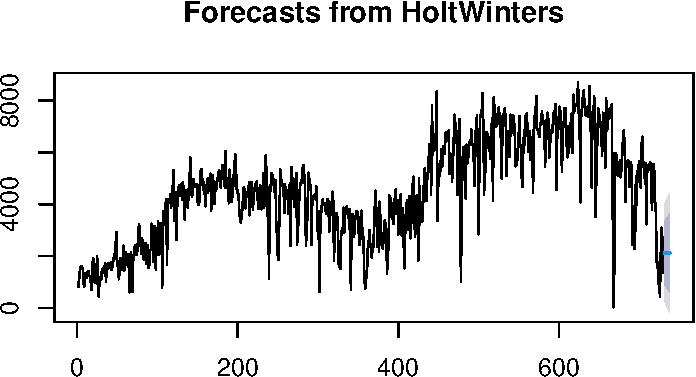
\includegraphics{prednaska2_HoltWinters_files/figure-pdf/unnamed-chunk-8-1.pdf}

\begin{Shaded}
\begin{Highlighting}[]
\NormalTok{forecast}\SpecialCharTok{:::}\FunctionTok{plot.forecast}\NormalTok{(countBikeHWforecast)}
\end{Highlighting}
\end{Shaded}

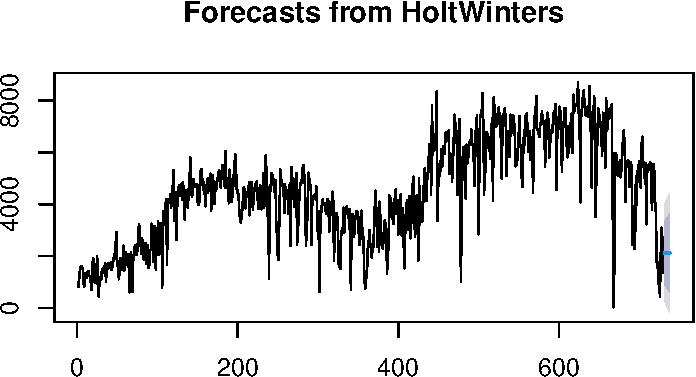
\includegraphics{prednaska2_HoltWinters_files/figure-pdf/unnamed-chunk-9-1.pdf}

Predpovede na 7 dní sú tu znázornené modrou čiarou, 80 \% interval
predpovedí viac tmavším sivým tieňom a 95 \% interval predpovedí beldším
sivým tieňom.

\subsection{Holt Winters prognózovanie s odstránenou trendovou
zložkou}\label{holt-winters-prognuxf3zovanie-s-odstruxe1nenou-trendovou-zloux17ekou}

Predpoveď časového radu požičiavania bicyklov v prípade, že povôdný rad
vyhladíme 30 dňovým jednoduchým kĺzavým priemerom:

\begin{Shaded}
\begin{Highlighting}[]
\NormalTok{countBikeSMA30 }\OtherTok{\textless{}{-}} \FunctionTok{SMA}\NormalTok{(countBike,}\AttributeTok{n=}\DecValTok{30}\NormalTok{)}
\FunctionTok{tail}\NormalTok{(countBikeSMA30,}\AttributeTok{n=}\DecValTok{10}\NormalTok{)}
\end{Highlighting}
\end{Shaded}

\begin{verbatim}
Time Series:
Start = 722 
End = 731 
Frequency = 1 
 [1] 4746.167 4675.400 4630.167 4583.133 4428.267 4366.767 4294.600 4161.867
 [9] 4032.800 3950.733
\end{verbatim}

\begin{Shaded}
\begin{Highlighting}[]
\NormalTok{countBikeNoTrend }\OtherTok{\textless{}{-}}\NormalTok{ countBike }\SpecialCharTok{{-}}\NormalTok{ countBikeSMA30}
\FunctionTok{tail}\NormalTok{(countBikeNoTrend,}\AttributeTok{n=}\DecValTok{10}\NormalTok{)}
\end{Highlighting}
\end{Shaded}

\begin{verbatim}
Time Series:
Start = 722 
End = 731 
Frequency = 1 
 [1] -2997.167 -2888.400 -3710.167 -3570.133 -3987.267 -2252.767 -1199.600
 [8] -2820.867 -2236.800 -1221.733
\end{verbatim}

\begin{Shaded}
\begin{Highlighting}[]
\FunctionTok{plot.ts}\NormalTok{(countBikeNoTrend)}
\end{Highlighting}
\end{Shaded}

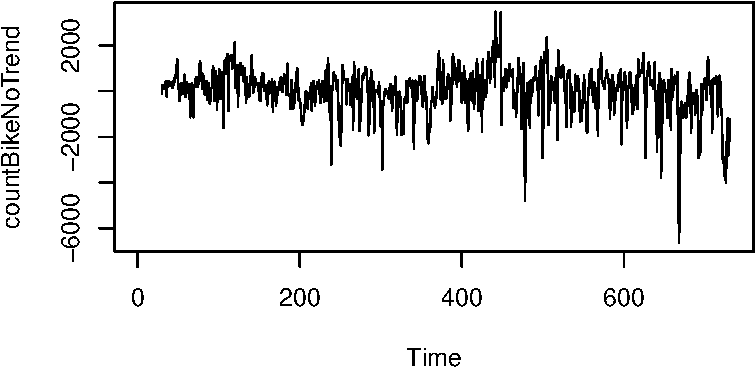
\includegraphics{prednaska2_HoltWinters_files/figure-pdf/unnamed-chunk-10-1.pdf}

\begin{Shaded}
\begin{Highlighting}[]
\NormalTok{countBikeNoTrendHW }\OtherTok{\textless{}{-}} \FunctionTok{HoltWinters}\NormalTok{(}\FunctionTok{subset}\NormalTok{(countBikeNoTrend, }\AttributeTok{start=}\DecValTok{30}\NormalTok{), }\AttributeTok{beta=}\ConstantTok{FALSE}\NormalTok{, }\AttributeTok{gamma=}\ConstantTok{FALSE}\NormalTok{)}
\NormalTok{countBikeNoTrendHWforecast }\OtherTok{\textless{}{-}}\NormalTok{ forecast}\SpecialCharTok{:::}\FunctionTok{forecast.HoltWinters}\NormalTok{(countBikeNoTrendHW, }\AttributeTok{h=}\DecValTok{7}\NormalTok{)}
\NormalTok{countBikeNoTrendHWforecast}
\end{Highlighting}
\end{Shaded}

\begin{verbatim}
    Point Forecast     Lo 80     Hi 80     Lo 95      Hi 95
732       -2095.39 -3320.816 -869.9639 -3969.517 -221.26258
733       -2095.39 -3353.882 -836.8982 -4020.087 -170.69292
734       -2095.39 -3386.101 -804.6793 -4069.362 -121.41834
735       -2095.39 -3417.535 -773.2453 -4117.436  -73.34416
736       -2095.39 -3448.239 -742.5415 -4164.393  -26.38670
737       -2095.39 -3478.261 -712.5192 -4210.308   19.52842
738       -2095.39 -3507.645 -683.1350 -4255.248   64.46768
\end{verbatim}

\begin{Shaded}
\begin{Highlighting}[]
\NormalTok{forecast}\SpecialCharTok{:::}\FunctionTok{plot.forecast}\NormalTok{(countBikeNoTrendHWforecast)}
\end{Highlighting}
\end{Shaded}

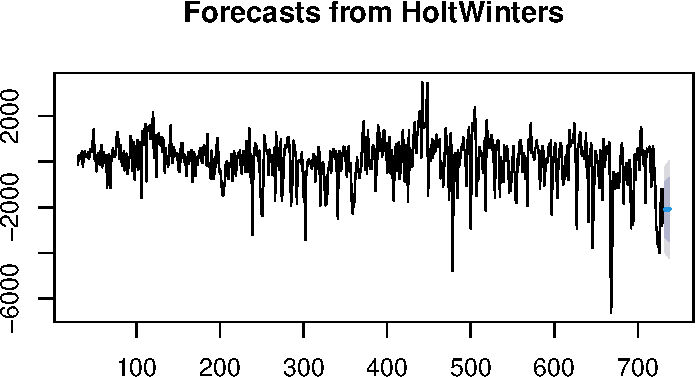
\includegraphics{prednaska2_HoltWinters_files/figure-pdf/unnamed-chunk-10-2.pdf}

\begin{Shaded}
\begin{Highlighting}[]
\FunctionTok{subset}\NormalTok{(countBike, }\AttributeTok{start=}\DecValTok{724}\NormalTok{)}
\end{Highlighting}
\end{Shaded}

\begin{verbatim}
Time Series:
Start = 724 
End = 731 
Frequency = 1 
[1]  920 1013  441 2114 3095 1341 1796 2729
\end{verbatim}

\begin{Shaded}
\begin{Highlighting}[]
\FunctionTok{subset}\NormalTok{(countBikeSMA30, }\AttributeTok{start=}\DecValTok{724}\NormalTok{)}
\end{Highlighting}
\end{Shaded}

\begin{verbatim}
Time Series:
Start = 724 
End = 731 
Frequency = 1 
[1] 4630.167 4583.133 4428.267 4366.767 4294.600 4161.867 4032.800 3950.733
\end{verbatim}

Potom od pôvodných hodnôt časového radu uložených v premennej
``countBike'' odpočítame hodnoty kĺzavého priemeru uložených v premennej
``countBikeSMA30'' a dostaneme nový časový rad z pôvodného, ktorý bol
očistený od trendovej zložky a je uložený v premennej
``countBikeNoTrend''. Nový časový trend náhodne kolíše okolo hodnoty 0,
čo znamená kolísanie hodnôt okolo trendu teda hodnôt jednoduchého
kĺzavého priemeru.

\subsection{Holt Winters prognózovanie s Box Cox transformáciou
dát}\label{holt-winters-prognuxf3zovanie-s-box-cox-transformuxe1ciou-duxe1t}

Na pôvodný časový rad požičaných biczklov uplatníme BoxCos
transformáciu, kde uvažujeme lambdu=0, čo v skotočnosti je logaritmická
transformácia dát a vieme, že časový rad je nazáporný a všetky hodnoty
sú rôzne od nuly, potom môžme uplatniť danú transformáciu.

\begin{Shaded}
\begin{Highlighting}[]
\NormalTok{countBikeTransform }\OtherTok{\textless{}{-}}\NormalTok{ forecast}\SpecialCharTok{::}\FunctionTok{BoxCox}\NormalTok{(countBike,}\AttributeTok{lambda=}\DecValTok{0}\NormalTok{)}
\FunctionTok{plot.ts}\NormalTok{(countBikeTransform)}
\end{Highlighting}
\end{Shaded}

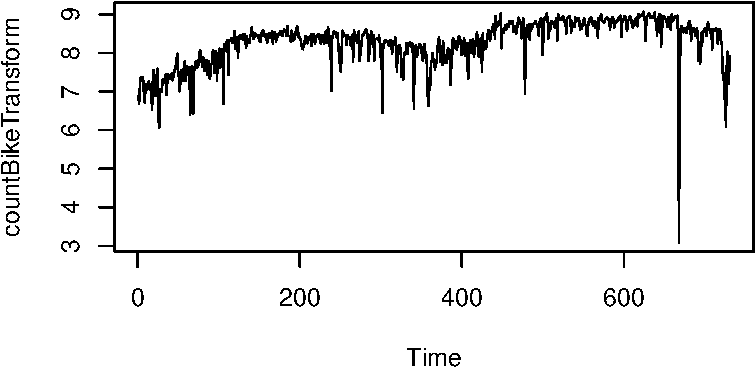
\includegraphics{prednaska2_HoltWinters_files/figure-pdf/unnamed-chunk-11-1.pdf}

\begin{Shaded}
\begin{Highlighting}[]
\NormalTok{countBikeTransformHW }\OtherTok{\textless{}{-}} \FunctionTok{HoltWinters}\NormalTok{(countBikeTransform,}\AttributeTok{beta=}\ConstantTok{FALSE}\NormalTok{, }\AttributeTok{gamma=}\ConstantTok{FALSE}\NormalTok{)}
\NormalTok{countBikeTransformHW}\SpecialCharTok{$}\NormalTok{SSE}
\end{Highlighting}
\end{Shaded}

\begin{verbatim}
[1] 98.21021
\end{verbatim}

\begin{Shaded}
\begin{Highlighting}[]
\NormalTok{countBikeTransformHWforecast }\OtherTok{\textless{}{-}}\NormalTok{ forecast}\SpecialCharTok{:::}\FunctionTok{forecast.HoltWinters}\NormalTok{(countBikeTransformHW, }\AttributeTok{h=}\DecValTok{7}\NormalTok{)}
\NormalTok{countBikeTransformHWforecast}
\end{Highlighting}
\end{Shaded}

\begin{verbatim}
    Point Forecast    Lo 80    Hi 80    Lo 95    Hi 95
732       7.547625 7.077270 8.017979 6.828280 8.266970
733       7.547625 7.065362 8.029888 6.810068 8.285182
734       7.547625 7.053741 8.041509 6.792295 8.302955
735       7.547625 7.042387 8.052863 6.774931 8.320319
736       7.547625 7.031283 8.063967 6.757948 8.337302
737       7.547625 7.020412 8.074837 6.741323 8.353927
738       7.547625 7.009762 8.085488 6.725034 8.370216
\end{verbatim}

\begin{Shaded}
\begin{Highlighting}[]
\NormalTok{forecast}\SpecialCharTok{:::}\FunctionTok{plot.forecast}\NormalTok{(countBikeTransformHWforecast)}
\end{Highlighting}
\end{Shaded}

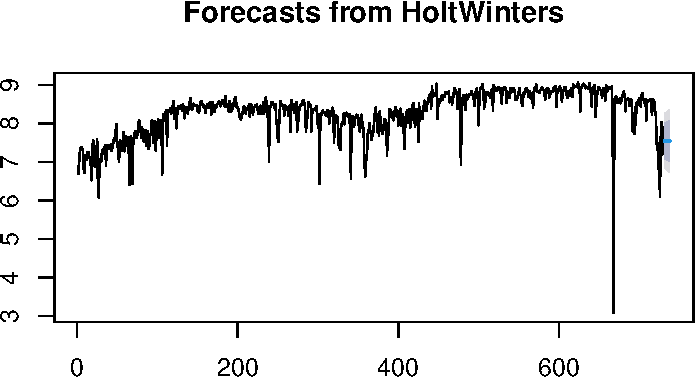
\includegraphics{prednaska2_HoltWinters_files/figure-pdf/unnamed-chunk-11-2.pdf}

\subsection{Chyba prognózy}\label{chyba-prognuxf3zy}

Chyby prognózy sa vypočítajú ako pozorované hodnoty mínus predpovedané
hodnoty pre každý časový bod. Chyby predpovede môžeme vypočítať len pre
časové obdobie, ktoré pokrýva náš pôvodný časový rad. Ako už bolo
uvedené, jedným z meradiel presnosti predpovedného modelu je súčet
štvorcov chýb (SSE) pre chyby predpovede vo vzorke.

Chyby predpovede vo vzorke sú uložené v pomenovanom prvku ``residuals''
premennej zoznamu vrátenej funkciou forecast.HoltWinters(). Ak sa
predpovedný model nedá zlepšiť, nemali by existovať žiadne korelácie
medzi chybami predpovede pre po sebe nasledujúce predpovede. Inými
slovami, ak existujú korelácie medzi chybami predpovedí pre po sebe
nasledujúce predpovede, je pravdepodobné, že jednoduché predpovede s
exponenciálnym vyhladzovaním by sa dali zlepšiť inou predpovednou
technikou.

Aby sme zistili, či je to tak, môžeme získať korelogram chýb prognóz vo
vzorke pre oneskorenia 1-20. Korelogram chýb prognózy môžeme vypočítať
pomocou funkcie ``acf()'' v jazyku R. Na určenie maximálneho
oneskorenia, na ktoré sa chceme pozrieť, použijeme parameter ``lag.max''
v funkcii acf().

Napríklad na výpočet korelogramu chýb predpovede vo vzorke pre dňové
údaje požičiavania bicyklov pre oneskorenia 1-20 zadáme:

\begin{Shaded}
\begin{Highlighting}[]
\FunctionTok{acf}\NormalTok{(}\FunctionTok{subset}\NormalTok{(countBikeHWforecast}\SpecialCharTok{$}\NormalTok{residuals,}\AttributeTok{start=}\DecValTok{2}\NormalTok{), }\AttributeTok{lag.max=}\DecValTok{20}\NormalTok{)}
\end{Highlighting}
\end{Shaded}

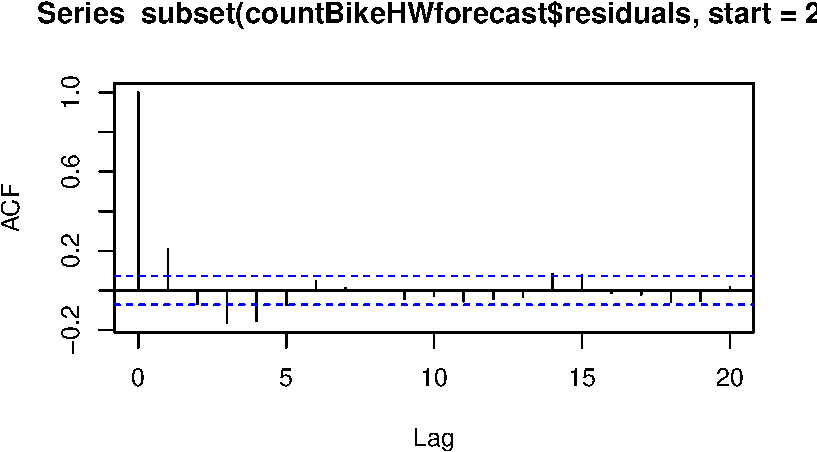
\includegraphics{prednaska2_HoltWinters_files/figure-pdf/unnamed-chunk-12-1.pdf}

Z korelogramu vzorky vidíte, že autokorelácia pri oneskorení 1 a 3
presahuje hranice významnosti. Ak chceme otestovať, či existuje významný
dôkaz nenulovej korelácie pri oneskoreniach 1 až 20, môžeme vykonať
Ljung-Boxov test. To sa dá urobiť v programe R pomocou funkcie
``Box.test()''. Maximálne oneskorenie, na ktoré sa chceme pozrieť, sa
špecifikuje pomocou parametra ``lag'' vo funkcii Box.test(). Napríklad,
ak chceme otestovať, či existujú nenulové autokorelácie pri
oneskoreniach 1-20, pre chyby predpovede vo vzorke požičaných bicyklov
zadáme:

\begin{Shaded}
\begin{Highlighting}[]
 \FunctionTok{Box.test}\NormalTok{(}\FunctionTok{subset}\NormalTok{(countBikeHWforecast}\SpecialCharTok{$}\NormalTok{residuals,}\AttributeTok{start=}\DecValTok{2}\NormalTok{), }\AttributeTok{lag=}\DecValTok{20}\NormalTok{, }\AttributeTok{type=}\StringTok{"Ljung{-}Box"}\NormalTok{)}
\end{Highlighting}
\end{Shaded}

\begin{verbatim}

    Box-Ljung test

data:  subset(countBikeHWforecast$residuals, start = 2)
X-squared = 98.84, df = 20, p-value = 2.03e-12
\end{verbatim}

V tomto prípade je Ljung-Boxova testovacia štatistika 98,84 a p-hodnota
je 2.03e-12, takže existuje dôkaz nenulovej autokorelácie v chybách
prognózy vo vzorke s oneskorením 1-20.

Aby sme si boli istí, že prognostický model nemožno zlepšiť, je tiež
dobré skontrolovať, či sú chyby prognózy normálne rozdelené so strednou
hodnotou nula a konštantným rozptylom. Na overenie, či chyby prognózy
majú konštantný rozptyl, môžeme urobiť časový graf chýb prognózy vo
vzorke:

\begin{Shaded}
\begin{Highlighting}[]
\FunctionTok{plot.ts}\NormalTok{(}\FunctionTok{subset}\NormalTok{(countBikeHWforecast}\SpecialCharTok{$}\NormalTok{residuals,}\AttributeTok{start=}\DecValTok{2}\NormalTok{))}
\end{Highlighting}
\end{Shaded}

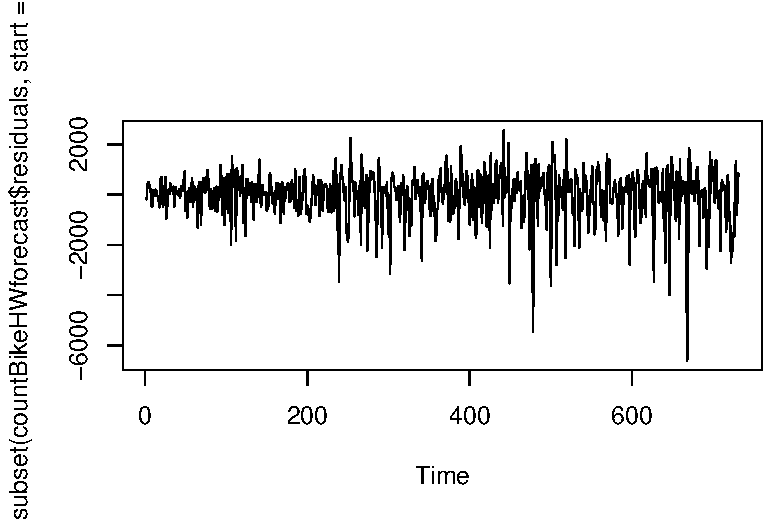
\includegraphics{prednaska2_HoltWinters_files/figure-pdf/unnamed-chunk-14-1.pdf}

Z grafu vyplýva, že chyby predpovedí vo vzorke majú v čase zrejme
približne konštantný rozptyl, hoci veľkosť výkyvov na začiatku časového
radu môže byť o niečo menšia ako v neskorších obdobiach.

Na overenie, či sú chyby predpovedí normálne rozdelené so strednou
hodnotou nula, môžeme vykresliť histogram chýb predpovedí s prekrytou
normálnou krivkou, ktorá má strednú hodnotu nula a rovnakú štandardnú
odchýlku ako rozdelenie chýb predpovedí. Na tento účel môžeme definovať
funkciu R ``plotForecastErrors()'', ktorá je uvedená nižšie:

\begin{Shaded}
\begin{Highlighting}[]
\NormalTok{plotForecastErrors }\OtherTok{\textless{}{-}} \ControlFlowTok{function}\NormalTok{(forecasterrors)}
\NormalTok{  \{}
     \CommentTok{\# histogram rezidui:}
\NormalTok{     mybinsize }\OtherTok{\textless{}{-}} \FunctionTok{IQR}\NormalTok{(forecasterrors)}\SpecialCharTok{/}\DecValTok{4}
\NormalTok{     mysd   }\OtherTok{\textless{}{-}} \FunctionTok{sd}\NormalTok{(forecasterrors)}
\NormalTok{     mymin  }\OtherTok{\textless{}{-}} \FunctionTok{min}\NormalTok{(forecasterrors) }\SpecialCharTok{{-}}\NormalTok{ mysd}\SpecialCharTok{*}\DecValTok{5}
\NormalTok{     mymax  }\OtherTok{\textless{}{-}} \FunctionTok{max}\NormalTok{(forecasterrors) }\SpecialCharTok{+}\NormalTok{ mysd}\SpecialCharTok{*}\DecValTok{3}
     \CommentTok{\# generované štandardné normálne dáta s 0 priemerom a std 1}
\NormalTok{     mynorm }\OtherTok{\textless{}{-}} \FunctionTok{rnorm}\NormalTok{(}\DecValTok{10000}\NormalTok{, }\AttributeTok{mean=}\DecValTok{0}\NormalTok{, }\AttributeTok{sd=}\NormalTok{mysd)}
\NormalTok{     mymin2 }\OtherTok{\textless{}{-}} \FunctionTok{min}\NormalTok{(mynorm)}
\NormalTok{     mymax2 }\OtherTok{\textless{}{-}} \FunctionTok{max}\NormalTok{(mynorm)}
     \ControlFlowTok{if}\NormalTok{ (mymin2 }\SpecialCharTok{\textless{}}\NormalTok{ mymin) \{ mymin }\OtherTok{\textless{}{-}}\NormalTok{ mymin2 \}}
     \ControlFlowTok{if}\NormalTok{ (mymax2 }\SpecialCharTok{\textgreater{}}\NormalTok{ mymax) \{ mymax }\OtherTok{\textless{}{-}}\NormalTok{ mymax2 \}}
     \CommentTok{\# červen sú reziduá a modrým sú normálne rozdelené dáta}
\NormalTok{     mybins }\OtherTok{\textless{}{-}} \FunctionTok{seq}\NormalTok{(mymin, mymax, mybinsize)}
     \FunctionTok{hist}\NormalTok{(forecasterrors, }\AttributeTok{col=}\StringTok{"red"}\NormalTok{, }\AttributeTok{freq=}\ConstantTok{FALSE}\NormalTok{, }\AttributeTok{breaks=}\NormalTok{mybins)}
     \CommentTok{\# freq=FALSE zaistí, že obsah pod histogramom bude rovný  1}
\NormalTok{     myhist }\OtherTok{\textless{}{-}} \FunctionTok{hist}\NormalTok{(mynorm, }\AttributeTok{plot=}\ConstantTok{FALSE}\NormalTok{, }\AttributeTok{breaks=}\NormalTok{mybins)}
     \FunctionTok{points}\NormalTok{(myhist}\SpecialCharTok{$}\NormalTok{mids, myhist}\SpecialCharTok{$}\NormalTok{density, }\AttributeTok{type=}\StringTok{"l"}\NormalTok{, }\AttributeTok{col=}\StringTok{"blue"}\NormalTok{, }\AttributeTok{lwd=}\DecValTok{2}\NormalTok{)}
\NormalTok{\}}

\FunctionTok{plotForecastErrors}\NormalTok{(}\FunctionTok{subset}\NormalTok{(countBikeHWforecast}\SpecialCharTok{$}\NormalTok{residuals,}\AttributeTok{start=}\DecValTok{2}\NormalTok{))}
\end{Highlighting}
\end{Shaded}

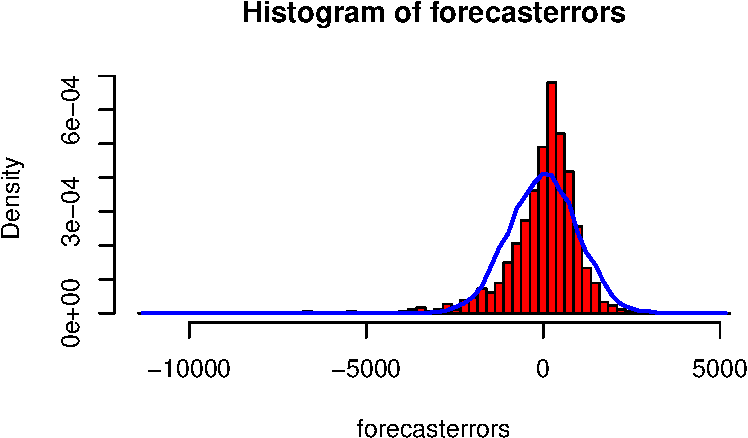
\includegraphics{prednaska2_HoltWinters_files/figure-pdf/unnamed-chunk-15-1.pdf}

\begin{Shaded}
\begin{Highlighting}[]
\FunctionTok{shapiro.test}\NormalTok{(}\FunctionTok{subset}\NormalTok{(countBikeHWforecast}\SpecialCharTok{$}\NormalTok{residuals,}\AttributeTok{start=}\DecValTok{2}\NormalTok{))}
\end{Highlighting}
\end{Shaded}

\begin{verbatim}

    Shapiro-Wilk normality test

data:  subset(countBikeHWforecast$residuals, start = 2)
W = 0.90756, p-value < 2.2e-16
\end{verbatim}

Z grafu vyplýva, že rozdelenie chýb predpovede je približne v strede
nuly a je viac-menej normálne rozložené, hoci sa zdá, že v porovnaní s
normálnou krivkou je mierne vychýlené doprava. Pravé skreslenie je však
relatívne malé, a preto je pravdepodobné, že chyby predpovede sú
normálne rozdelené so strednou hodnotou nula.

Ljungov-Boxov test ukázal, že v chybách prognózy vo vzorke existuje
dôkaz nenulovej autokorelácie a zdá sa, že rozdelenie chýb prognózy je
normálne rozdelené so strednou hodnotou nula. Výsledky naznačujú, že
jednoduchá metóda exponenciálneho vyhladzovania neposkytuje primeraný
predpovedný model pre požičiavanie bicyklov, ktorý pravdepodobne vieme
inými metódami zlepšiť.

Predpoklad ,že v chybách predpovede neexistujú autokorelácie, na ktorej
boli založené 80 \% a 95 \% intervaly predpovedí sú neplatné. Prepoklad
normality máme len graficky zatiaľ oevrenú a mali bz sme použiť test
normality. Sahpiro=Wilk normality test ukázal, že dáta nie sú normlané
rozdelené. Preto musíme otestovať stacionaritu radu a použiť ine
nástroje časových raodv na určenie predpovede.

\part{Model Bieleho Šumu (white noise) a Náhodná Prechádzka (Random
walk)}

\chapter{Model bieleho šumu (white noise
(WN))}\label{model-bieleho-ux161umu-white-noise-wn}

Model bieleho šumu (WN) je základným modelom časového radu. Je tiež
základom pre zložitejšie modely, ktoré budeme posudzovať. Zameriame sa
na najjednoduchšiu formu bieleho šumu, nezávislé a identicky rozdelené
údaje. Model bieleho šumu je najjednoduchším príkladom stacionárneho
procesu, ktorý má:

\begin{itemize}
\tightlist
\item
  fixnú, konštantnú strednú hodnotu,
\item
  fixný, konštantný rozptyl a
\item
  žiadnu koreláciu v čase.
\end{itemize}

Pozrime sa na niekoľko grafov časových radov bieleho šumu.

\begin{figure}[H]

{\centering 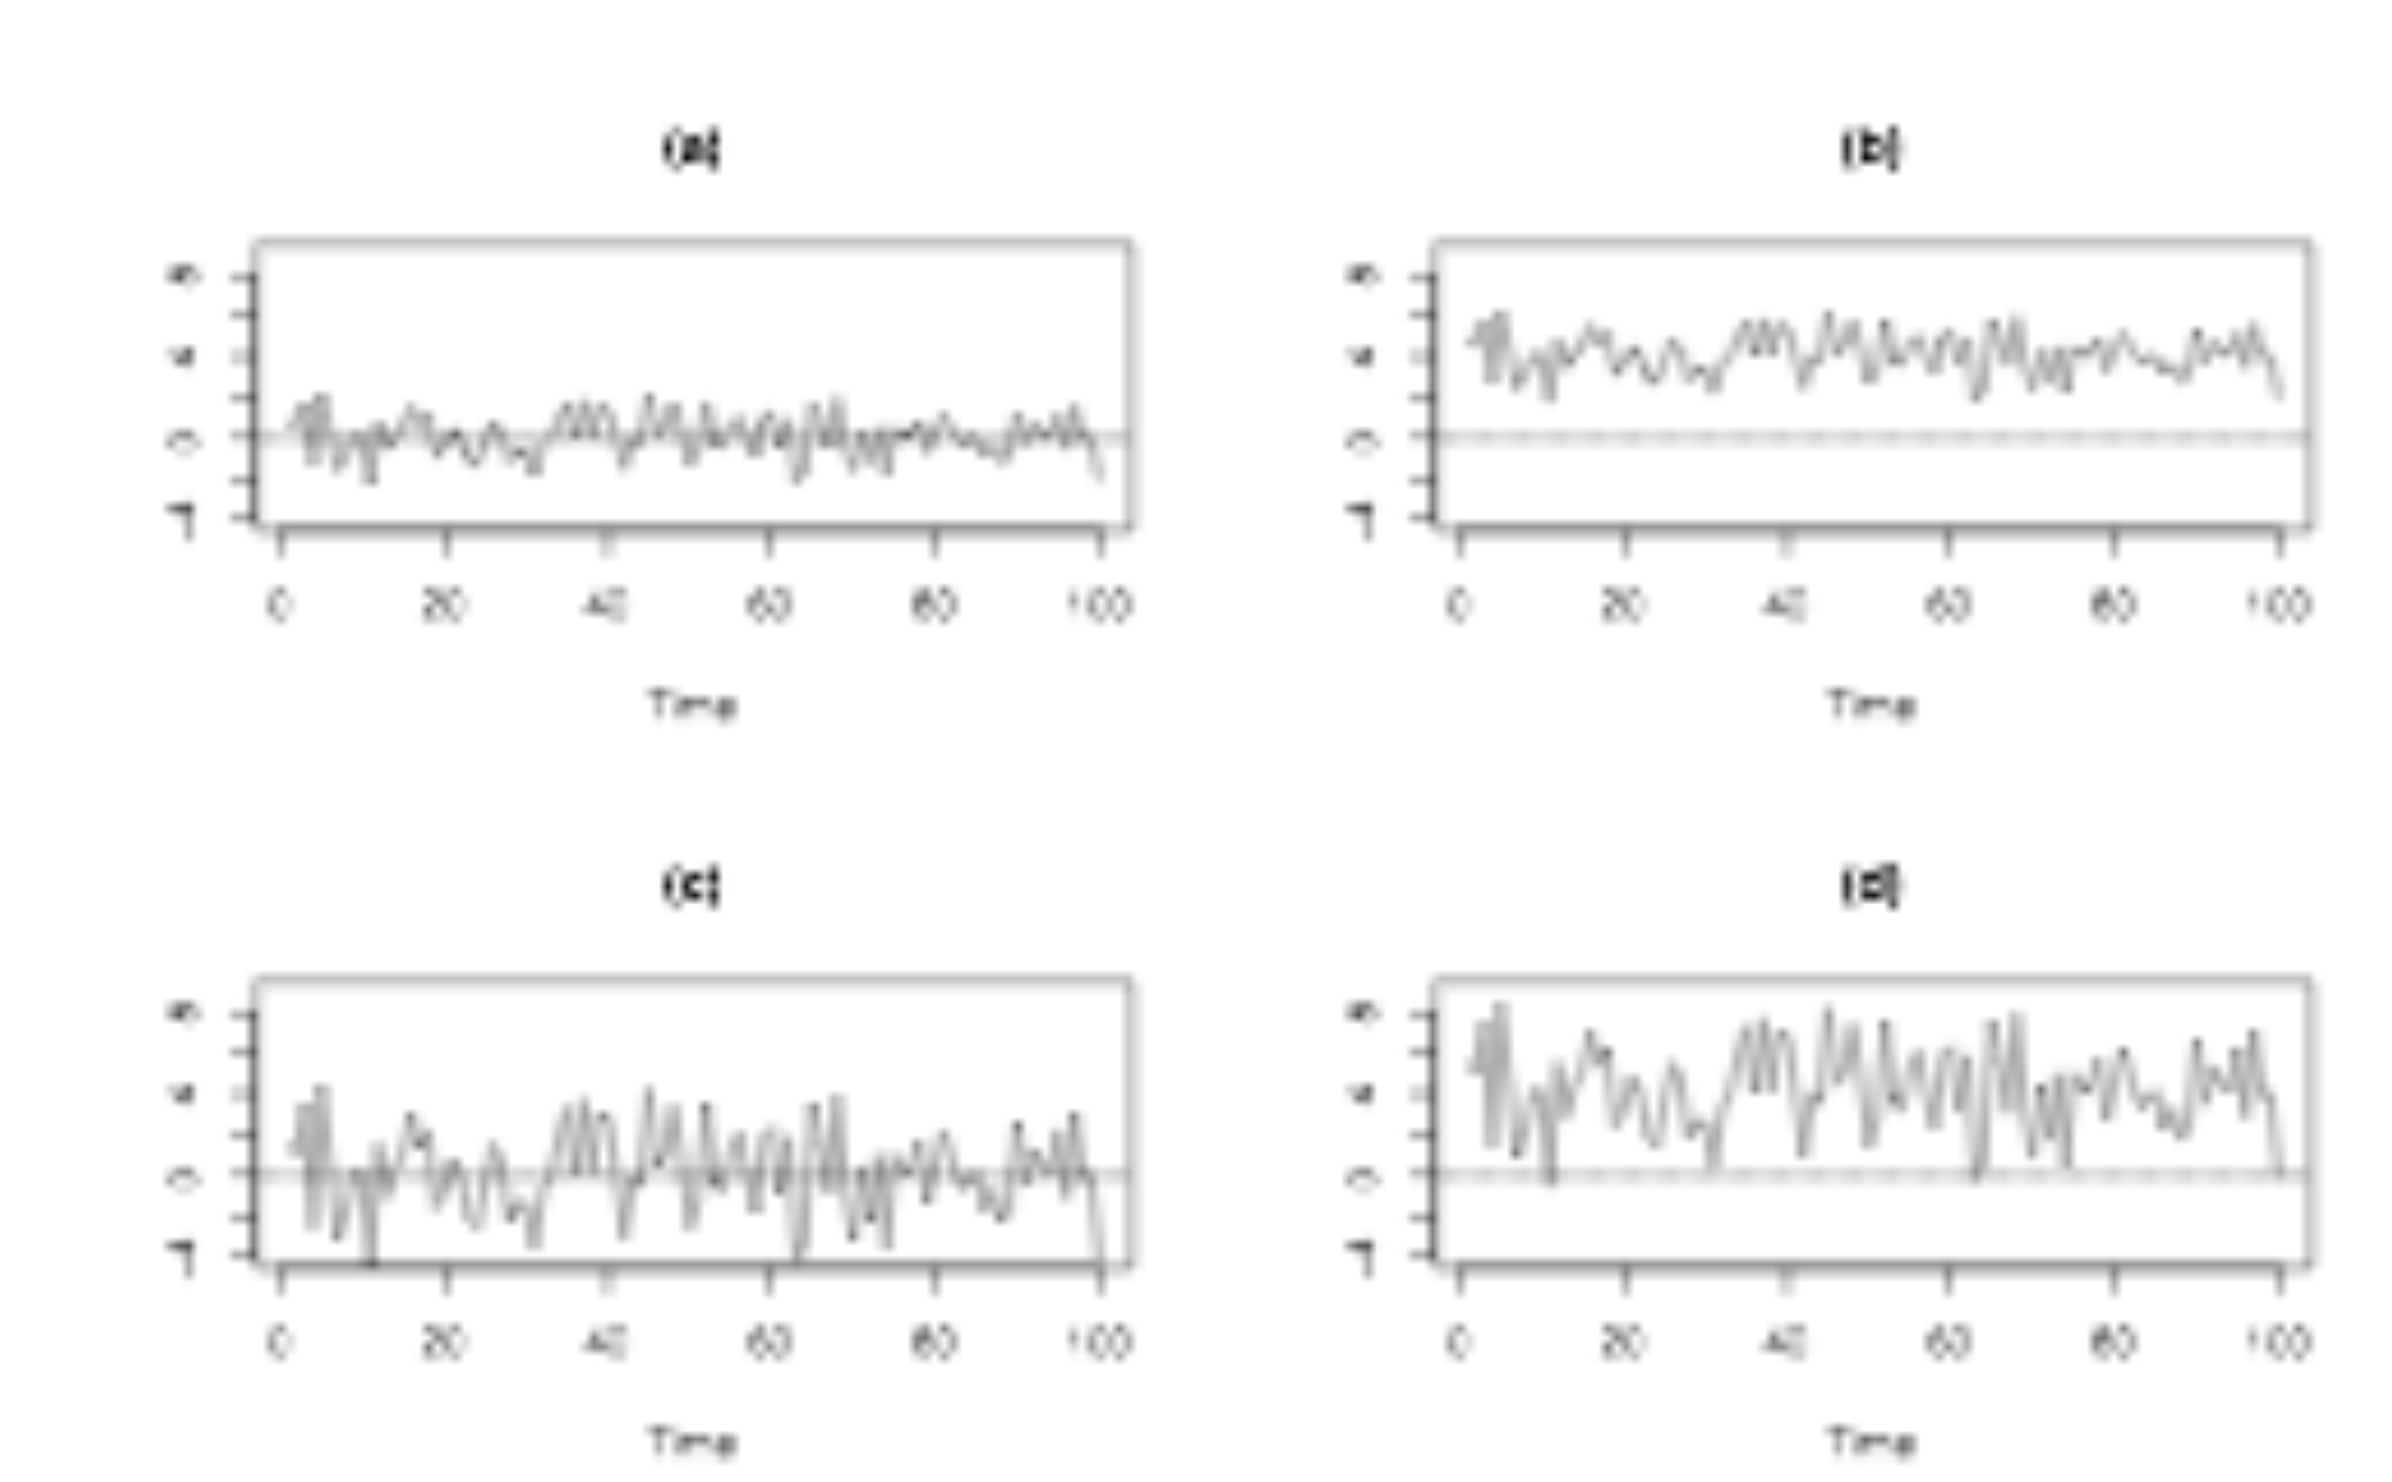
\includegraphics{wn1.png}

}

\caption{Obrázok 1. 4 grafy Bieleho šumu.}

\end{figure}%

Na grafe A si všimnite, že v údajoch nie je žiadny vzor ani korelácia v
čase. Na grafe B sa rad posunul nahor, čo naznačuje väčší priemer, ale v
údajoch stále nie sú žiadne vzory. Na grafe C má rad väčšiu vertikálnu
variabilitu, čo znamená väčší rozptyl, ale v údajoch stále nie sú žiadne
vzory. A napokon v prípade garfu D má rad väčší priemer aj väčší
rozptyl, ale opäť nemá jasný vzor alebo trend v čase. Všetky štyri
obrázky sú príkladmi časových radov bieleho šumu.

Teraz sa pozrieme na štyri nové grafy. Otázka je : Ktorý z nich je biely
šum?

\begin{figure}[H]

{\centering 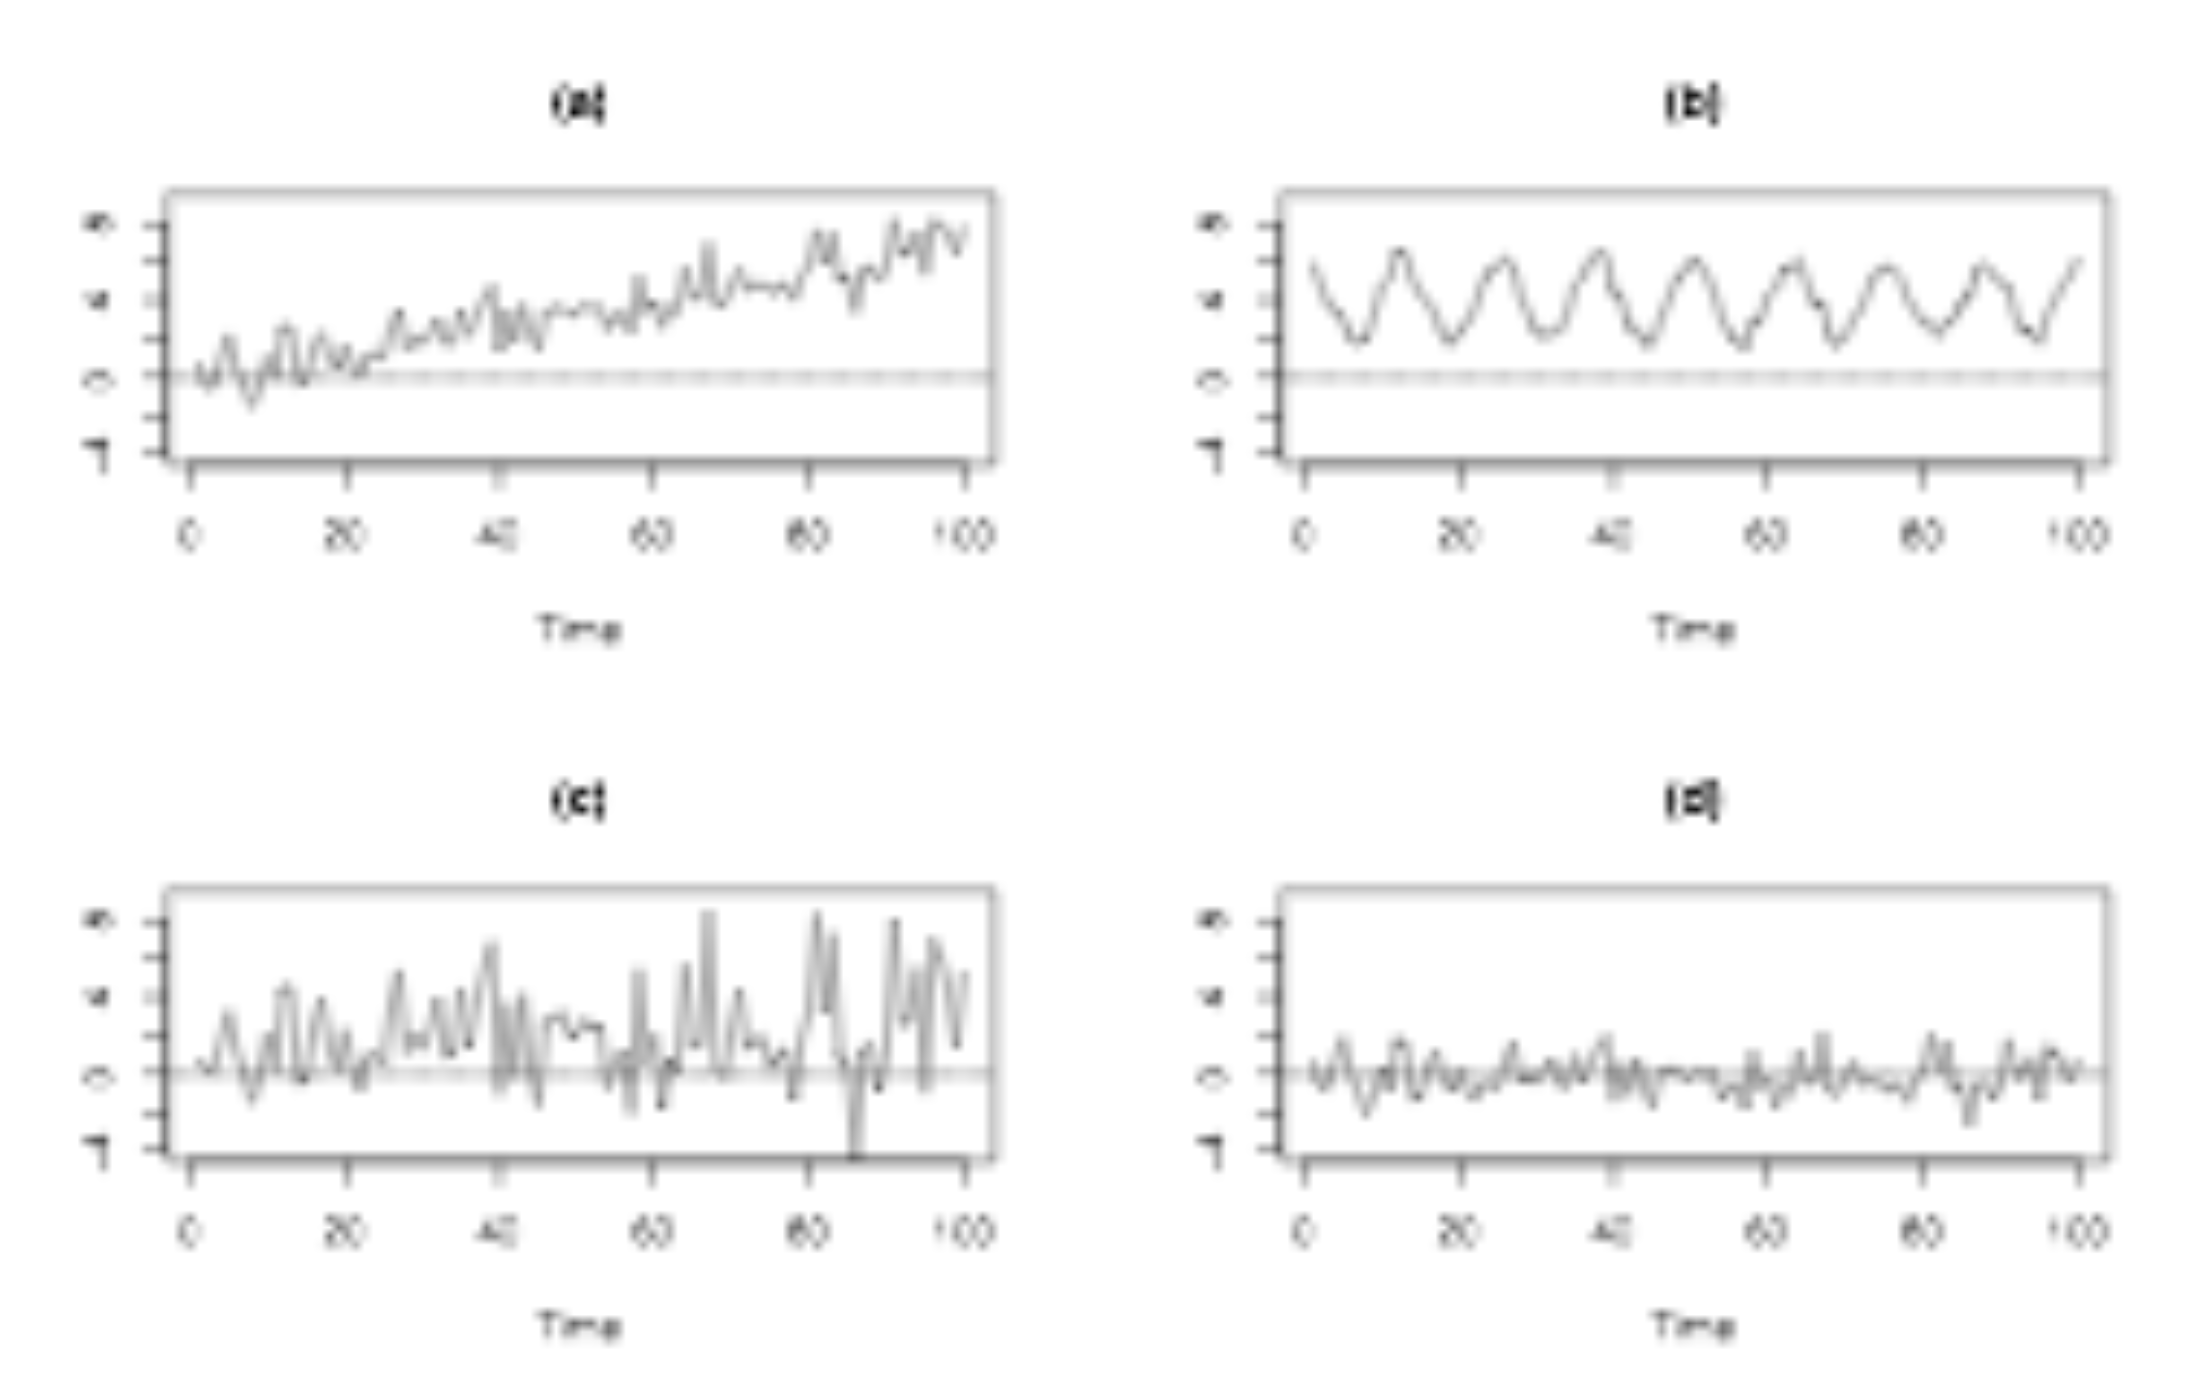
\includegraphics{wn2.png}

}

\caption{Obrázok 2. Ktorý graf je Biely šum?.}

\end{figure}%

Graf A má stúpajúci časový trend, jeho priemer nie je v čase konštantný,
takže to nie je biely šum. Graf B má jasný periodický vzor s pevnou
dĺžkou cyklu, ktorý sa opakuje približne každých 12 pozorovaní. Jeho
stredná hodnota tiež nie je v čase konštantná, takže nejde o biely šum.
Graf C vykazuje väčšiu variabilitu vpravo ako vľavo, to znamená, že sa
zdá, že rozptyl v čase rastie. Keďže rozptyl nie je konštantný, tiež
nejde o biely šum. Zostáva graf D, ktorý má podľa všetkého konštantnú
strednú hodnotu aj rozptyl a žiadne jasné vzory alebo koreláciu v čase,
takže spĺňa predpoklady modelu bieleho šumu.

\subsection{Simulácia modelu bieleho
šumu}\label{simuluxe1cia-modelu-bieleho-ux161umu}

Na simuláciu časového radu bieleho šumu možno použiť funkciu
arima.sim(). ARIMA je skratka pre triedu modelov autoregresných
integrovaných kĺzavých priemerov, ktoré budeme v tomto predmete uvažovať
(budeme sa venovať v ARIMA modelom neskorších cvičeniach). V stručnosti
si len uvedieme, čo znamenajú parametre modelu ARIMA, ktoré použijeme
nižšie uvedenej funkcie. Model ARIMA(p, d, q) má tri časti, a to
autoregresný rád p, rád integrácie (alebo diferencovania) d a rád
kĺzavého priemeru q. Každú z týchto častí čoskoro podrobne popíšeme v
neskorších cvičeniach, ale teraz si všimnime, že model ARIMA(0, 0, 0),
t. j. so všetkými týmito zložkami nulovými, je jednoducho model bieleho
šumu.

Je to veľmi široká trieda modelov časových radov, ktorá zahŕňa biely šum
ako špeciálny prípad. Na špecifikáciu modelu bieleho šumu použijeme
špeciálny rád špecifický pre biely šum, ako je znázornené v kóde
(list(order = c(0, 0, 0)). Simuluje sa rad s n rovné päťdesiatim
pozorovaniam. Niektoré simulované hodnoty bieleho šumu sú zobrazené
pomocou funkcie head.

\begin{Shaded}
\begin{Highlighting}[]
\FunctionTok{set.seed}\NormalTok{(}\DecValTok{123}\NormalTok{)}
\CommentTok{\# Simulácia n = 50 pozorovaní modelu bieleho šumu}
\NormalTok{bielySum1 }\OtherTok{\textless{}{-}} \FunctionTok{arima.sim}\NormalTok{(}\AttributeTok{model =} \FunctionTok{list}\NormalTok{(}\AttributeTok{order =} \FunctionTok{c}\NormalTok{(}\DecValTok{0}\NormalTok{, }\DecValTok{0}\NormalTok{, }\DecValTok{0}\NormalTok{)), }\AttributeTok{n =} \DecValTok{50}\NormalTok{)}
\FunctionTok{head}\NormalTok{(bielySum1)}
\end{Highlighting}
\end{Shaded}

\begin{verbatim}
[1] -0.56047565 -0.23017749  1.55870831  0.07050839  0.12928774  1.71506499
\end{verbatim}

Celý rad simulovaného bieleho šumu je znázornený na obrázku. Predvolený
priemer a štandardná odchýlka pre rad sú nula, resp. jedna.

\begin{Shaded}
\begin{Highlighting}[]
\FunctionTok{ts.plot}\NormalTok{(bielySum1)}
\end{Highlighting}
\end{Shaded}

\includegraphics{prednaska3_NahodnaPrechadzkaStacionarita_files/figure-pdf/unnamed-chunk-2-1.pdf}

Simuláciu môžete zopakovať so strednou hodnotou rovnou štyrom a
štandardnou odchýlkou rovnou 2 tak, že ich pridáte ako ďalšie argumenty,
ako je znázornené v kóde. Na obrázku vidíme, že simulované hodnoty
oscilujú okolo hodnoty 4 (priemer) na vertikálnej osi.

\begin{Shaded}
\begin{Highlighting}[]
\NormalTok{bielySum2 }\OtherTok{\textless{}{-}} \FunctionTok{arima.sim}\NormalTok{(}\AttributeTok{model =} \FunctionTok{list}\NormalTok{(}\AttributeTok{order =} \FunctionTok{c}\NormalTok{(}\DecValTok{0}\NormalTok{, }\DecValTok{0}\NormalTok{, }\DecValTok{0}\NormalTok{)), }\AttributeTok{n =} \DecValTok{50}\NormalTok{, }\AttributeTok{mean=}\DecValTok{4}\NormalTok{,}\AttributeTok{sd=}\DecValTok{2}\NormalTok{)}
\FunctionTok{head}\NormalTok{(bielySum2)}
\end{Highlighting}
\end{Shaded}

\begin{verbatim}
[1] 4.506637 3.942906 3.914259 6.737205 3.548458 7.032941
\end{verbatim}

\begin{Shaded}
\begin{Highlighting}[]
\FunctionTok{ts.plot}\NormalTok{(bielySum2)}
\end{Highlighting}
\end{Shaded}

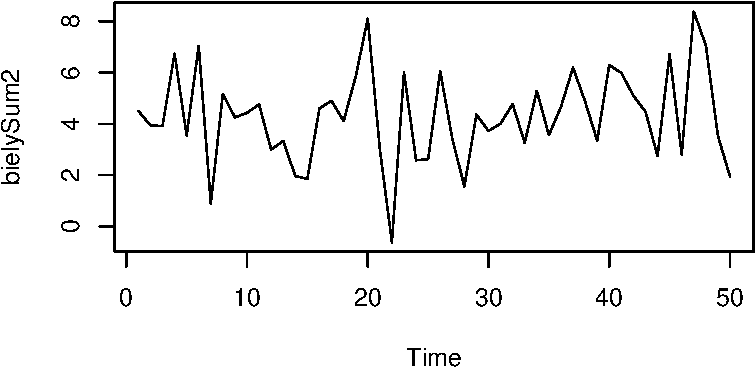
\includegraphics{prednaska3_NahodnaPrechadzkaStacionarita_files/figure-pdf/unnamed-chunk-3-1.pdf}

\subsection{Odhad modelu bieleho
šumu}\label{odhad-modelu-bieleho-ux161umu}

Nakoniec môžeme pre daný časový rad odhadnúť model bieleho šumu. Na to
použijeme funkciu arima(), pričom najprv poskytneme údaje (premenná
bielySum1), potom nastavíme rády modelu, ako je znázornené v kóde
(list(order = c(0, 0, 0)).

\begin{Shaded}
\begin{Highlighting}[]
\FunctionTok{arima}\NormalTok{(bielySum1, }\AttributeTok{order =} \FunctionTok{c}\NormalTok{(}\DecValTok{0}\NormalTok{, }\DecValTok{0}\NormalTok{, }\DecValTok{0}\NormalTok{))}
\end{Highlighting}
\end{Shaded}

\begin{verbatim}

Call:
arima(x = bielySum1, order = c(0, 0, 0))

Coefficients:
      intercept
         0.0344
s.e.     0.1296

sigma^2 estimated as 0.8401:  log likelihood = -66.59,  aic = 137.18
\end{verbatim}

\begin{Shaded}
\begin{Highlighting}[]
\FunctionTok{mean}\NormalTok{(bielySum1)}
\end{Highlighting}
\end{Shaded}

\begin{verbatim}
[1] 0.03440355
\end{verbatim}

\begin{Shaded}
\begin{Highlighting}[]
\FunctionTok{var}\NormalTok{(bielySum1)}
\end{Highlighting}
\end{Shaded}

\begin{verbatim}
[1] 0.8572352
\end{verbatim}

\begin{Shaded}
\begin{Highlighting}[]
\FunctionTok{sqrt}\NormalTok{(}\FunctionTok{var}\NormalTok{(bielySum1))}
\end{Highlighting}
\end{Shaded}

\begin{verbatim}
[1] 0.92587
\end{verbatim}

Táto funkcia vráti odhad strednej hodnoty alebo interceptu, ktorý je pre
tento časový rad približne 0.0344, približnú štandardnú chybu tohto
odhadu strednej hodnoty, v tomto prípade 0.1296, a odhad rozptylu alebo
sigma kvadrát, ktorý bol 0.8401. Odhadovaná štandardná odchýlka je
samozrejme odmocninou z tohto odhadu rozptylu. Alternatívne môžete
použiť funkcie mean() a var() na priamy odhad parametrov strednej
hodnoty 0.0344 a rozptylu modelu bieleho šumu 0.8572. Podobne môžeme
spraviť aj pre druhý rad bieleho šumu reprezentovaný premenou bielySum2:

\begin{Shaded}
\begin{Highlighting}[]
\FunctionTok{arima}\NormalTok{(bielySum2, }\AttributeTok{order =} \FunctionTok{c}\NormalTok{(}\DecValTok{0}\NormalTok{, }\DecValTok{0}\NormalTok{, }\DecValTok{0}\NormalTok{))}
\end{Highlighting}
\end{Shaded}

\begin{verbatim}

Call:
arima(x = bielySum2, order = c(0, 0, 0))

Coefficients:
      intercept
         4.2928
s.e.     0.2535

sigma^2 estimated as 3.214:  log likelihood = -100.13,  aic = 204.27
\end{verbatim}

\begin{Shaded}
\begin{Highlighting}[]
\FunctionTok{mean}\NormalTok{(bielySum2)}
\end{Highlighting}
\end{Shaded}

\begin{verbatim}
[1] 4.292817
\end{verbatim}

\begin{Shaded}
\begin{Highlighting}[]
\FunctionTok{var}\NormalTok{(bielySum2)}
\end{Highlighting}
\end{Shaded}

\begin{verbatim}
[1] 3.279339
\end{verbatim}

\begin{Shaded}
\begin{Highlighting}[]
\FunctionTok{sqrt}\NormalTok{(}\FunctionTok{var}\NormalTok{(bielySum2))}
\end{Highlighting}
\end{Shaded}

\begin{verbatim}
[1] 1.810894
\end{verbatim}

\section{Náhodná prechádzka (Random
walk)}\label{nuxe1hodnuxe1-prechuxe1dzka-random-walk}

Náhodná prechádzka alebo RW je jednoduchý príklad nestabilného alebo
nestacionárneho procesu a má tieto vlastnosti:

\begin{itemize}
\tightlist
\item
  Nemá určenú strednú hodnotu ani rozptyl.
\item
  Vykazuje veľmi silnú závislosť v čase, pričom každé pozorovanie úzko
  súvisí s jeho bezprostrednými susedmi.
\item
  Jeho zmeny alebo prírastky sa však riadia procesom bieleho šumu, ktorý
  je stabilný a stacionárny.
\end{itemize}

Pozrime sa na niektoré grafy časových radov náhodnej prechádzky.

\begin{figure}[H]

{\centering 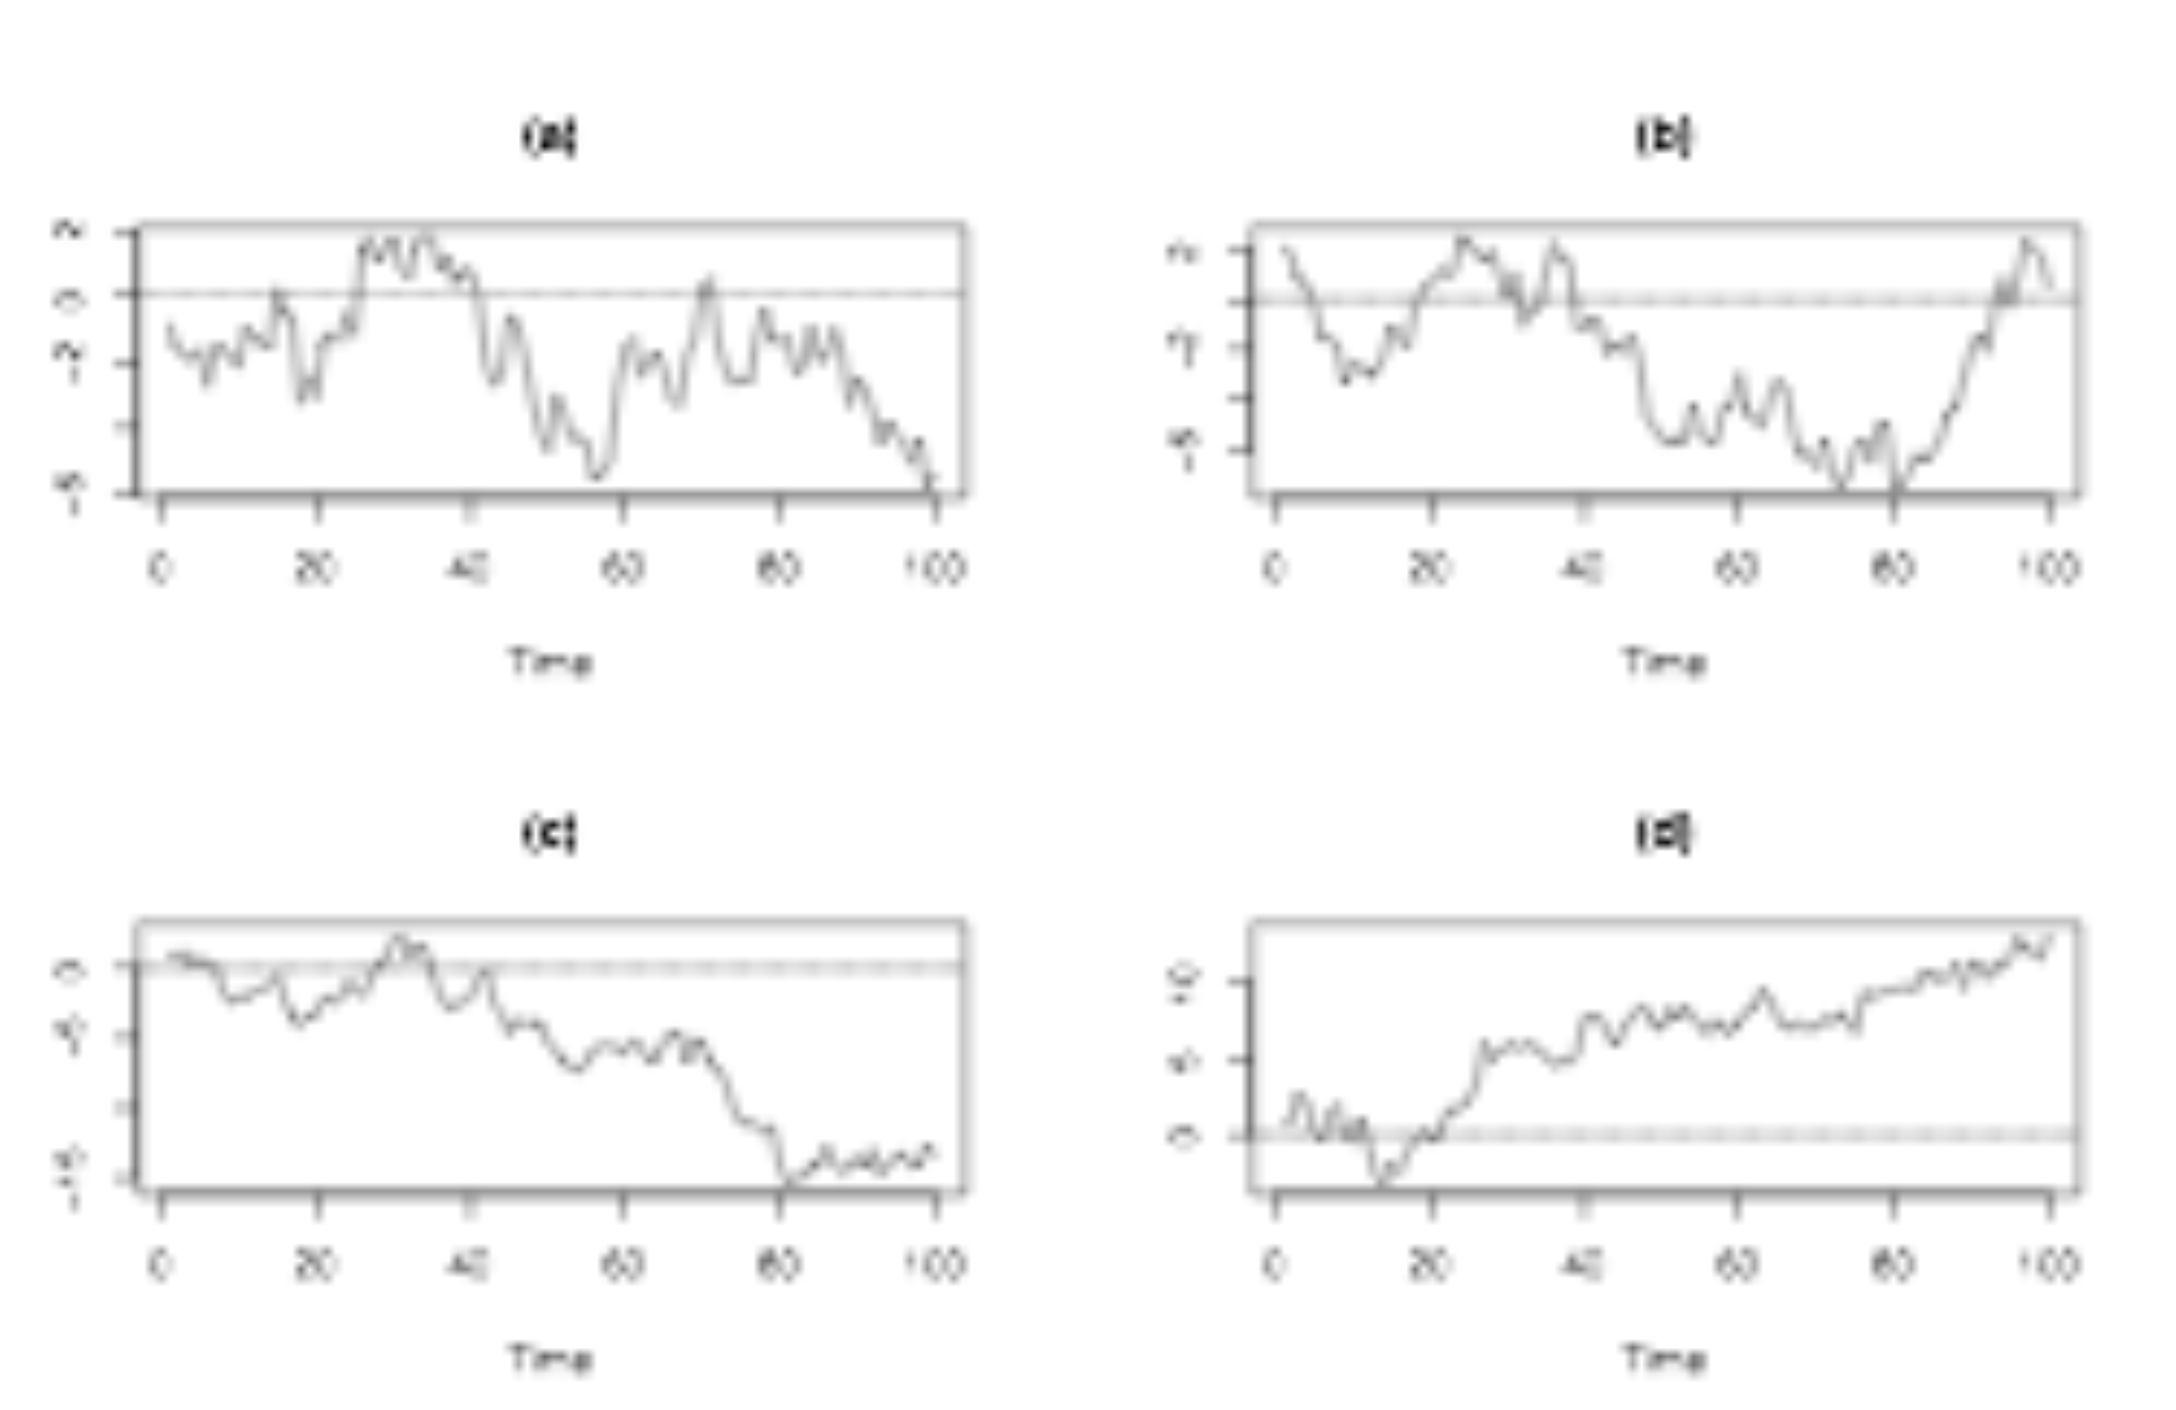
\includegraphics{rw.png}

}

\caption{Obrázok 3. Ktorý graf je Biely šum?.}

\end{figure}%

Na grafe A si všimnite, že v rade je silná stálosť. Susedné pozorovania
sú podobné a náhodne sa objavujú krátke trendy smerom nahor a nadol.
Niekoľkokrát pretína prerušovanú vodorovnú nulovú čiaru. Graf B vykazuje
mnohé z tých istých znakov. Graf C začína blízko nuly, ale potom sa
pohybuje smerom nadol, zatiaľ čo graf D začína blízko nuly, ale potom sa
pohybuje smerom nahor. Každý z nich je časovým radom náhodnej
prechádzky.

Teraz sa pozrime na model náhodnej prechádzky. Je definovaný rekurzívne.

\(Dnes = Včera + Šum\)

Dnešné alebo aktuálne pozorovanie sa rovná včerajšiemu alebo
predchádzajúcemu pozorovaniu plus šum alebo chyba. Viac formálny zápis:

\(Y_t = Y_{t-1} + \epsilon_t\)

Táto chyba \(\epsilon_t\) je konkrétne biely šum so strednou hodnotou
(priemerom) 0. V praxi si simulácia časového radu náhodnej prechádzky
vyžaduje:

\begin{itemize}
\tightlist
\item
  Počiatočný bod \(Y_0\).
\item
  Model náhodnej prechádzky má len jeden parameter, ktorým je rozptyl
  bieleho šumu \(\sigma^2_{\epsilon}\).
\end{itemize}

Vzhľadom na bod \(Y_0\) a prvý člen bieleho šumu vygenerujete prvé
pozorovanie Náhodnej prechádzky ako \(Y_1 = Y_0 + \epsilon_1\) a potom
pokračujete k časovému indexu dva, kde \(Y_2 = Y_1 + \epsilon_2\) .
Často sa pre jednoduchosť ako počiatočný bod \(Y_0\) používa hodnota
nula. Musíte si dopredu nagenerovať aj hodnoty bieleho šumu, čo sme už
urobili vyššie.

Výrazy v náhodnej prechádzke sa dajú usporiadať ako rad prvej
diferencie. Tu vidíte, že rozdiel medzi aktuálnym pozorovaním \(Y_t\) a
predchádzajúcim pozorovaním \(Y_{t-1}\)

\(Y_t - Y_{t-1} =  \epsilon_t\)

sa rovná členovi šumu \(\epsilon_t\). To znamená, že rozdielový rad
alebo rad zmien je biely šum.

\subsection{Simulácia modelu náhodnej
prechádzky}\label{simuluxe1cia-modelu-nuxe1hodnej-prechuxe1dzky}

Najprv si zadefinujeme rad náhodnej prechádzky a premennej dáme názov
randomWalk. Budeme mať časovú radu o dĺžke 50, pretože biely šum 1 mal
toľko hodnôt. Rad inicializujeme nulovými hodnotami. Vypočítame prvý
člen radu náhodnej prechádzky keďže sme už definovali \(Y_0\) ako prvú
hodnotu v rade, ktorá bola inicializovaná hodnotou nula. Potom využijeme
iteračný cyklus ``for'' a dorátame jednotlivé časové kroky od 2 až po 50
rekurzívne.

\begin{Shaded}
\begin{Highlighting}[]
\NormalTok{randomWalk }\OtherTok{\textless{}{-}} \FunctionTok{rep}\NormalTok{(}\DecValTok{0}\NormalTok{,}\FunctionTok{length}\NormalTok{(bielySum1))}
\CommentTok{\#vypočítame prvý člen radu náhodnej prechádzky  }
\NormalTok{randomWalk[}\DecValTok{1}\NormalTok{] }\OtherTok{\textless{}{-}}\NormalTok{ randomWalk[}\DecValTok{1}\NormalTok{] }\SpecialCharTok{+}\NormalTok{ bielySum1[}\DecValTok{1}\NormalTok{]}
\ControlFlowTok{for}\NormalTok{ (i }\ControlFlowTok{in} \DecValTok{2}\SpecialCharTok{:}\FunctionTok{length}\NormalTok{(bielySum1)) \{}
\NormalTok{    randomWalk[i] }\OtherTok{\textless{}{-}}\NormalTok{ randomWalk[i}\DecValTok{{-}1}\NormalTok{] }\SpecialCharTok{+}\NormalTok{ bielySum1[i]}
\NormalTok{\}}
\FunctionTok{plot}\NormalTok{(randomWalk,}\AttributeTok{type=}\StringTok{"b"}\NormalTok{, }\AttributeTok{xlab=}\StringTok{"čas"}\NormalTok{,}\AttributeTok{ylab=}\StringTok{"hodnoty náhodnej prechádzky"}\NormalTok{, }\AttributeTok{main=}\StringTok{"Náhodná prechádzka s použitím bieleho šumu 1"}\NormalTok{)}
\end{Highlighting}
\end{Shaded}

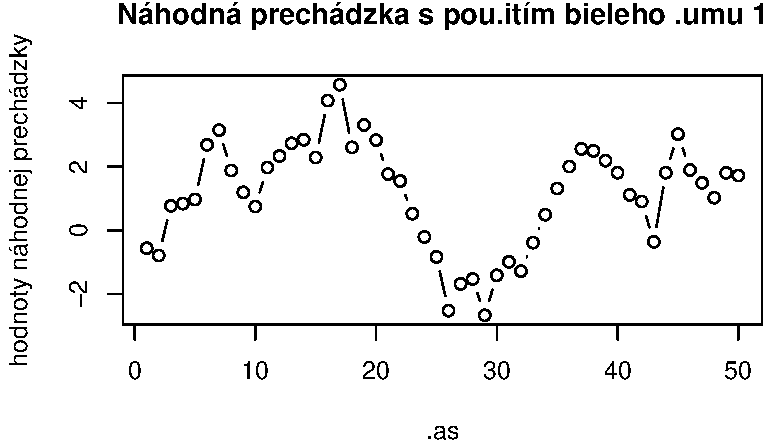
\includegraphics{prednaska3_NahodnaPrechadzkaStacionarita_files/figure-pdf/unnamed-chunk-6-1.pdf}

Na obrázku genereovaného R kódom vidíme simulovanú nahodnú prechádzku.

Ak začnete s časovým radom náhodná prechádzka (randomWalk), a použijete
funkciu diff() v R na výpočet rozdielového radu, výsledok tejto
jednoduchej transformácie uvidíte, že rozdiely alebo zmeny či prírastky
časového radu randomWalk sú radom bieleho šumu 1. Teraz sa pozrieme na
priebeh prvých diferencií.

\begin{Shaded}
\begin{Highlighting}[]
\NormalTok{prveDiffRW }\OtherTok{\textless{}{-}} \FunctionTok{diff}\NormalTok{(randomWalk)}
\FunctionTok{plot}\NormalTok{(prveDiffRW,}\AttributeTok{type=}\StringTok{"b"}\NormalTok{,}\AttributeTok{xlab=}\StringTok{"čas"}\NormalTok{,}\AttributeTok{ylab=}\StringTok{"hodnoty prvých differencií náhodnej prechádzky"}\NormalTok{,}\AttributeTok{main=}\StringTok{"Prvé differencie náhodnej prechádzky s použitím bieleho šumu 1"}\NormalTok{)}
\end{Highlighting}
\end{Shaded}

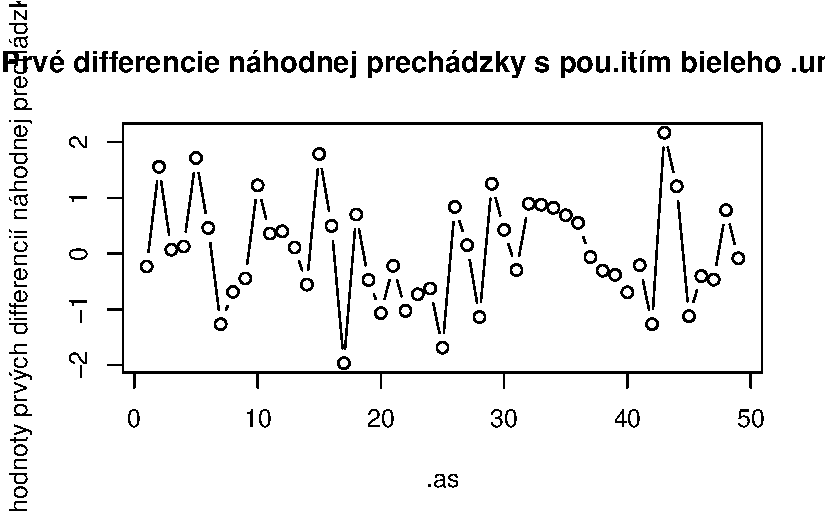
\includegraphics{prednaska3_NahodnaPrechadzkaStacionarita_files/figure-pdf/unnamed-chunk-7-1.pdf}

\begin{Shaded}
\begin{Highlighting}[]
\FunctionTok{mean}\NormalTok{(prveDiffRW)}
\end{Highlighting}
\end{Shaded}

\begin{verbatim}
[1] 0.04654394
\end{verbatim}

\begin{Shaded}
\begin{Highlighting}[]
\FunctionTok{var}\NormalTok{(prveDiffRW)}
\end{Highlighting}
\end{Shaded}

\begin{verbatim}
[1] 0.8675713
\end{verbatim}

\begin{Shaded}
\begin{Highlighting}[]
\FunctionTok{sqrt}\NormalTok{(}\FunctionTok{var}\NormalTok{(prveDiffRW))}
\end{Highlighting}
\end{Shaded}

\begin{verbatim}
[1] 0.9314351
\end{verbatim}

\begin{Shaded}
\begin{Highlighting}[]
\FunctionTok{mean}\NormalTok{(bielySum1[}\DecValTok{2}\SpecialCharTok{:}\DecValTok{50}\NormalTok{])}
\end{Highlighting}
\end{Shaded}

\begin{verbatim}
[1] 0.04654394
\end{verbatim}

\begin{Shaded}
\begin{Highlighting}[]
\FunctionTok{var}\NormalTok{(bielySum1[}\DecValTok{2}\SpecialCharTok{:}\DecValTok{50}\NormalTok{])}
\end{Highlighting}
\end{Shaded}

\begin{verbatim}
[1] 0.8675713
\end{verbatim}

Vidíme z výsledku, že rad prvých diferencíí náhodnej prechádzky má
priemer blízky nule a rozptzl blízky k 1.Graf naynačuje, že sa pôvodný
rad bieleho šumu 1 a prv0 differencie náhodnej prechádzky rovanjú. Chýba
nám prvý údaj lebo pri differenciácii vypadne prvý údaj.Teda overíme to
tak, že vypočitame priemer a štandardnú odhchýlku pre pozorovania 2 až
50 bieleho šumu 1 a dostávame tie isté hodnoty ako pre rad prvých
diferencií.

\subsection{Simulácia modelu náhodnej prechádzky s konštatným členom
(driftom)}\label{simuluxe1cia-modelu-nuxe1hodnej-prechuxe1dzky-s-konux161tatnuxfdm-ux10dlenom-driftom}

Model náhodnej prechádzky možno rozšíriť o koeficient driftu (posun,
pomalá zmena). Tým sa do rekurzívneho vzorca pridá konštanta C.

\(Y_t = C + Y_{t-1} + \epsilon_t\)

Náhodná prechádzka s driftom má dva parametre, driftovú konštantu C a
sigma-kvadrát rozptylu bieleho šumu \(\sigma^2_{\epsilon}\). Aký je prvý
diferenčný rad náhodnej prechádzky s driftom? Je to jednoducho konštanta
plus šum, čo je proces bieleho šumu so strednou hodnotou C.

\begin{Shaded}
\begin{Highlighting}[]
\NormalTok{c }\OtherTok{\textless{}{-}} \FloatTok{0.3}
\NormalTok{randomWalkDrift }\OtherTok{\textless{}{-}} \FunctionTok{rep}\NormalTok{(}\DecValTok{0}\NormalTok{,}\FunctionTok{length}\NormalTok{(bielySum1))}
\CommentTok{\#vypočítame prvý člen radu náhodnej prechádzky }
\NormalTok{randomWalkDrift[}\DecValTok{1}\NormalTok{] }\OtherTok{\textless{}{-}}\NormalTok{ randomWalkDrift[}\DecValTok{1}\NormalTok{] }\SpecialCharTok{+}\NormalTok{ bielySum1[}\DecValTok{1}\NormalTok{]}
\ControlFlowTok{for}\NormalTok{ (i }\ControlFlowTok{in} \DecValTok{2}\SpecialCharTok{:}\FunctionTok{length}\NormalTok{(bielySum1)) \{}
\NormalTok{    randomWalkDrift[i] }\OtherTok{\textless{}{-}}\NormalTok{ c }\SpecialCharTok{+}\NormalTok{ randomWalkDrift[i}\DecValTok{{-}1}\NormalTok{] }\SpecialCharTok{+}\NormalTok{ bielySum1[i]}
\NormalTok{\}}
\FunctionTok{plot}\NormalTok{(randomWalkDrift,}\AttributeTok{type=}\StringTok{"b"}\NormalTok{, }\AttributeTok{xlab=}\StringTok{"čas"}\NormalTok{,}\AttributeTok{ylab=}\StringTok{"hodnoty náhodnej prechádzky"}\NormalTok{, }\AttributeTok{main=}\StringTok{"Náhodná prechádzka s použitím bieleho šumu 1 a driftom c=0.3"}\NormalTok{)}
\end{Highlighting}
\end{Shaded}

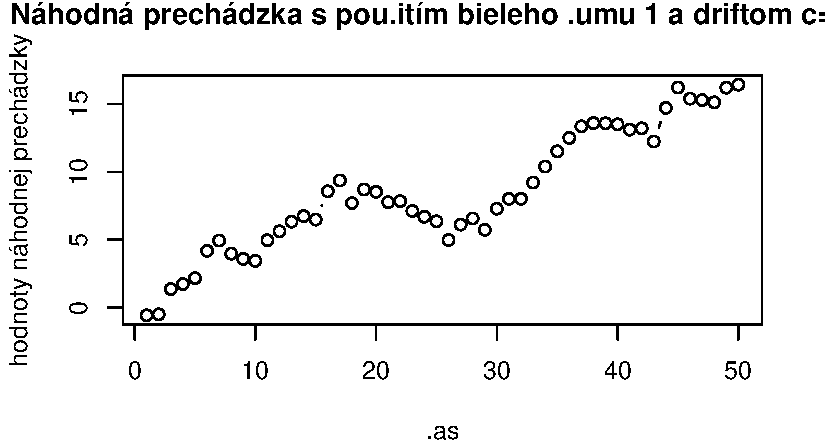
\includegraphics{prednaska3_NahodnaPrechadzkaStacionarita_files/figure-pdf/unnamed-chunk-8-1.pdf}

Vidíme, že konštanta c vlastne vytvára lineárny trend pre náhodnú
prechádzku s driftom. Kedže hodnoty bieleho šumu sú malé a pohybujú sa
od =2 do 2, časom je tam vidieť nejaký výkyv okolo rastúceho lineárneho
trendu, ale čím bude c väčšie tým budú výkyvy okolo trendu vidieť menej
lebo hodnota trednu pre daný časový bod je väčšia ako samotný biely šum.
Drift teda unáša hodnoty s lineaárnym trendom rastúcim smerom ak c je
kladné, klesajúcim ak c je záporné. Teraz urobme prvé differencie
náhodnej prechádzky s driftom.

\begin{Shaded}
\begin{Highlighting}[]
\NormalTok{prveDiffRWDrift }\OtherTok{\textless{}{-}} \FunctionTok{diff}\NormalTok{(randomWalkDrift)}
\FunctionTok{plot}\NormalTok{(prveDiffRWDrift,}\AttributeTok{type=}\StringTok{"b"}\NormalTok{,}\AttributeTok{xlab=}\StringTok{"čas"}\NormalTok{,}\AttributeTok{ylab=}\StringTok{"hodnoty prvých differencií náhodnej prechádzky s driftom c=0.3"}\NormalTok{,}\AttributeTok{main=}\StringTok{"Prvé differencie náhodnej prechádzky s použitím bieleho šumu 1"}\NormalTok{)}
\end{Highlighting}
\end{Shaded}

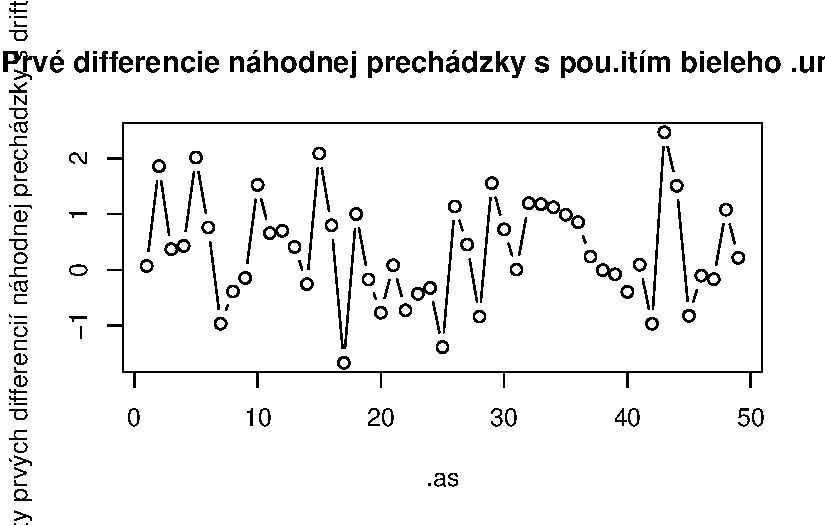
\includegraphics{prednaska3_NahodnaPrechadzkaStacionarita_files/figure-pdf/unnamed-chunk-9-1.pdf}

\begin{Shaded}
\begin{Highlighting}[]
\FunctionTok{mean}\NormalTok{(prveDiffRWDrift)}
\end{Highlighting}
\end{Shaded}

\begin{verbatim}
[1] 0.3465439
\end{verbatim}

\begin{Shaded}
\begin{Highlighting}[]
\FunctionTok{var}\NormalTok{(prveDiffRWDrift)}
\end{Highlighting}
\end{Shaded}

\begin{verbatim}
[1] 0.8675713
\end{verbatim}

\begin{Shaded}
\begin{Highlighting}[]
\FunctionTok{sqrt}\NormalTok{(}\FunctionTok{var}\NormalTok{(prveDiffRWDrift))}
\end{Highlighting}
\end{Shaded}

\begin{verbatim}
[1] 0.9314351
\end{verbatim}

\begin{Shaded}
\begin{Highlighting}[]
\FunctionTok{mean}\NormalTok{(bielySum1[}\DecValTok{2}\SpecialCharTok{:}\DecValTok{50}\NormalTok{])}
\end{Highlighting}
\end{Shaded}

\begin{verbatim}
[1] 0.04654394
\end{verbatim}

\begin{Shaded}
\begin{Highlighting}[]
\FunctionTok{var}\NormalTok{(bielySum1[}\DecValTok{2}\SpecialCharTok{:}\DecValTok{50}\NormalTok{])}
\end{Highlighting}
\end{Shaded}

\begin{verbatim}
[1] 0.8675713
\end{verbatim}

Takže vidíme, že prvé diferencie radu náhodnej prechádzky s driftom
c=0.3 je tiež proces bieleho šumu len priemerná hodnota nieje 0, a je
posunutá o konštantu c.~Teraz skúsme vygenerovať biely šum so strednou
hodnotou 0.3 a štandardnou odchýlkou 1.

\begin{Shaded}
\begin{Highlighting}[]
\NormalTok{bielySumDrift }\OtherTok{\textless{}{-}} \FunctionTok{arima.sim}\NormalTok{(}\AttributeTok{model =} \FunctionTok{list}\NormalTok{(}\AttributeTok{order =} \FunctionTok{c}\NormalTok{(}\DecValTok{0}\NormalTok{, }\DecValTok{0}\NormalTok{, }\DecValTok{0}\NormalTok{)), }\AttributeTok{n =} \DecValTok{50}\NormalTok{, }\AttributeTok{mean=}\FloatTok{0.3}\NormalTok{)}
\FunctionTok{head}\NormalTok{(bielySumDrift)}
\end{Highlighting}
\end{Shaded}

\begin{verbatim}
[1] -0.41040656  0.55688371  0.05330812 -0.04754260 -0.65161857  0.25497228
\end{verbatim}

\begin{Shaded}
\begin{Highlighting}[]
\FunctionTok{ts.plot}\NormalTok{(bielySumDrift)}
\end{Highlighting}
\end{Shaded}

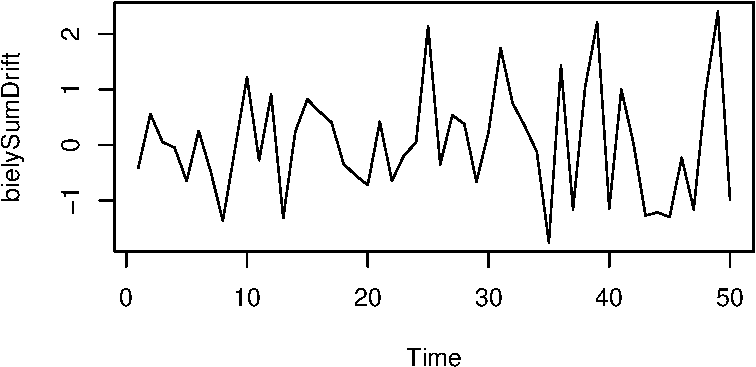
\includegraphics{prednaska3_NahodnaPrechadzkaStacionarita_files/figure-pdf/unnamed-chunk-10-1.pdf}

\begin{Shaded}
\begin{Highlighting}[]
\FunctionTok{mean}\NormalTok{(bielySumDrift)}
\end{Highlighting}
\end{Shaded}

\begin{verbatim}
[1] 0.04609957
\end{verbatim}

\begin{Shaded}
\begin{Highlighting}[]
\FunctionTok{var}\NormalTok{(bielySumDrift)}
\end{Highlighting}
\end{Shaded}

\begin{verbatim}
[1] 0.9787816
\end{verbatim}

\begin{Shaded}
\begin{Highlighting}[]
\FunctionTok{sqrt}\NormalTok{(}\FunctionTok{var}\NormalTok{(bielySumDrift))}
\end{Highlighting}
\end{Shaded}

\begin{verbatim}
[1] 0.9893339
\end{verbatim}

\begin{Shaded}
\begin{Highlighting}[]
\FunctionTok{arima}\NormalTok{(bielySumDrift, }\AttributeTok{order =} \FunctionTok{c}\NormalTok{(}\DecValTok{0}\NormalTok{, }\DecValTok{0}\NormalTok{, }\DecValTok{0}\NormalTok{))}
\end{Highlighting}
\end{Shaded}

\begin{verbatim}

Call:
arima(x = bielySumDrift, order = c(0, 0, 0))

Coefficients:
      intercept
         0.0461
s.e.     0.1385

sigma^2 estimated as 0.9592:  log likelihood = -69.91,  aic = 143.81
\end{verbatim}

Vidíme, že grafy prvých differencií a bieleho šumu s driftom s priemerom
0.3 a štandardnou odhýlkou 1 sa podobajú.Odhad priemeru bieleho šumu s
driftom presne nevyšiel na 0.3, ale je tam určitá chyba a teda v rámci
chybz sa nachádza aj hodnota 0.3. Nemohli sme drift zvoliť väčší lebo by
sme nevideli tie výkyvy okolo rastúceho trendu. Zvoľme si drift
napríklad 1 a uvidíme, že prvé differencie budú radou bieleho šumu s
priemerom 1.

\begin{Shaded}
\begin{Highlighting}[]
\NormalTok{c }\OtherTok{\textless{}{-}} \DecValTok{1}
\NormalTok{randomWalkDriftVelky }\OtherTok{\textless{}{-}} \FunctionTok{rep}\NormalTok{(}\DecValTok{0}\NormalTok{,}\FunctionTok{length}\NormalTok{(bielySum1))}
\CommentTok{\#vypočítame prvý člen radu náhodnej prechádzky }
\NormalTok{randomWalkDriftVelky[}\DecValTok{1}\NormalTok{] }\OtherTok{\textless{}{-}}\NormalTok{ randomWalkDriftVelky[}\DecValTok{1}\NormalTok{] }\SpecialCharTok{+}\NormalTok{ bielySum1[}\DecValTok{1}\NormalTok{]}
\ControlFlowTok{for}\NormalTok{ (i }\ControlFlowTok{in} \DecValTok{2}\SpecialCharTok{:}\FunctionTok{length}\NormalTok{(bielySum1)) \{}
\NormalTok{    randomWalkDriftVelky[i] }\OtherTok{\textless{}{-}}\NormalTok{ c }\SpecialCharTok{+}\NormalTok{ randomWalkDriftVelky[i}\DecValTok{{-}1}\NormalTok{] }\SpecialCharTok{+}\NormalTok{ bielySum1[i]}
\NormalTok{\}}
\FunctionTok{plot}\NormalTok{(randomWalkDriftVelky,}\AttributeTok{type=}\StringTok{"b"}\NormalTok{, }\AttributeTok{xlab=}\StringTok{"čas"}\NormalTok{,}\AttributeTok{ylab=}\StringTok{"hodnoty náhodnej prechádzky"}\NormalTok{, }\AttributeTok{main=}\StringTok{"Náhodná prechádzka s použitím bieleho šumu 1 a driftom c=1"}\NormalTok{)}
\end{Highlighting}
\end{Shaded}

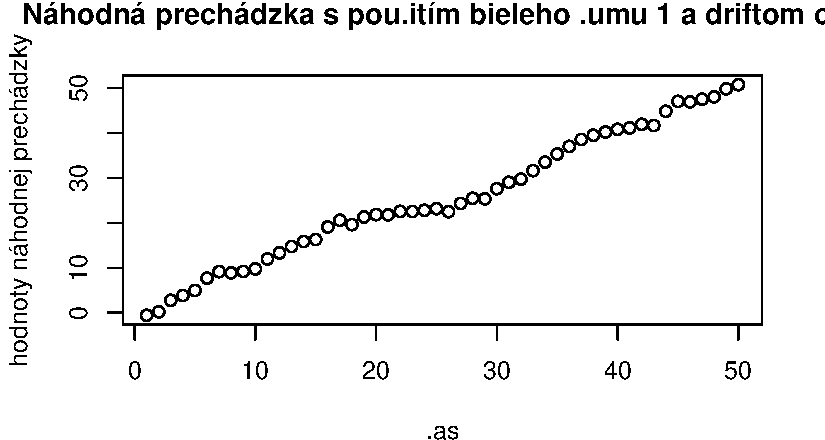
\includegraphics{prednaska3_NahodnaPrechadzkaStacionarita_files/figure-pdf/unnamed-chunk-11-1.pdf}

\begin{Shaded}
\begin{Highlighting}[]
\NormalTok{prveDiffRWDriftVelky }\OtherTok{\textless{}{-}} \FunctionTok{diff}\NormalTok{(randomWalkDriftVelky)}
\FunctionTok{plot}\NormalTok{(prveDiffRWDriftVelky,}\AttributeTok{type=}\StringTok{"b"}\NormalTok{,}\AttributeTok{xlab=}\StringTok{"čas"}\NormalTok{,}\AttributeTok{ylab=}\StringTok{"hodnoty prvých differencií náhodnej prechádzky s driftom c=1"}\NormalTok{,}\AttributeTok{main=}\StringTok{"Prvé differencie náhodnej prechádzky s použitím bieleho šumu 1"}\NormalTok{)}
\end{Highlighting}
\end{Shaded}

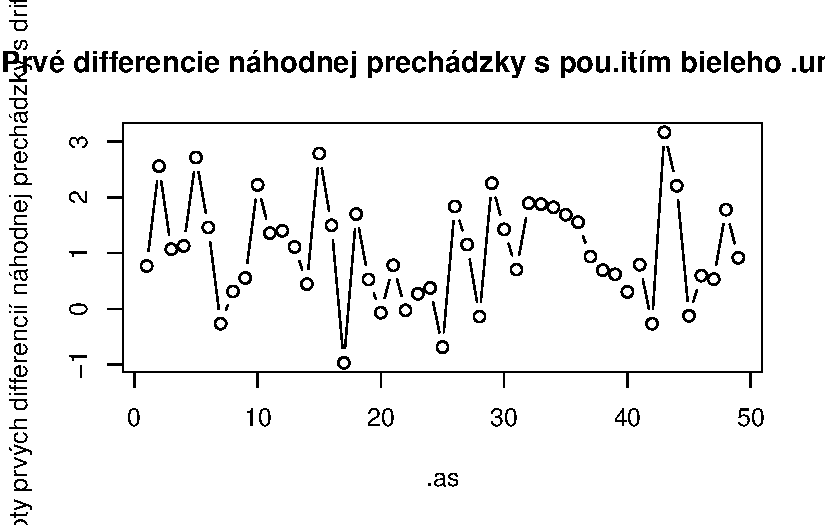
\includegraphics{prednaska3_NahodnaPrechadzkaStacionarita_files/figure-pdf/unnamed-chunk-11-2.pdf}

\begin{Shaded}
\begin{Highlighting}[]
\FunctionTok{mean}\NormalTok{(prveDiffRWDriftVelky)}
\end{Highlighting}
\end{Shaded}

\begin{verbatim}
[1] 1.046544
\end{verbatim}

\begin{Shaded}
\begin{Highlighting}[]
\FunctionTok{var}\NormalTok{(prveDiffRWDriftVelky)}
\end{Highlighting}
\end{Shaded}

\begin{verbatim}
[1] 0.8675713
\end{verbatim}

\begin{Shaded}
\begin{Highlighting}[]
\FunctionTok{sqrt}\NormalTok{(}\FunctionTok{var}\NormalTok{(prveDiffRWDriftVelky))}
\end{Highlighting}
\end{Shaded}

\begin{verbatim}
[1] 0.9314351
\end{verbatim}

\begin{Shaded}
\begin{Highlighting}[]
\FunctionTok{mean}\NormalTok{(bielySum1[}\DecValTok{2}\SpecialCharTok{:}\DecValTok{50}\NormalTok{])}
\end{Highlighting}
\end{Shaded}

\begin{verbatim}
[1] 0.04654394
\end{verbatim}

\begin{Shaded}
\begin{Highlighting}[]
\FunctionTok{var}\NormalTok{(bielySum1[}\DecValTok{2}\SpecialCharTok{:}\DecValTok{50}\NormalTok{])}
\end{Highlighting}
\end{Shaded}

\begin{verbatim}
[1] 0.8675713
\end{verbatim}

\begin{Shaded}
\begin{Highlighting}[]
\NormalTok{bielySumDriftVelky }\OtherTok{\textless{}{-}} \FunctionTok{arima.sim}\NormalTok{(}\AttributeTok{model =} \FunctionTok{list}\NormalTok{(}\AttributeTok{order =} \FunctionTok{c}\NormalTok{(}\DecValTok{0}\NormalTok{, }\DecValTok{0}\NormalTok{, }\DecValTok{0}\NormalTok{)), }\AttributeTok{n =} \DecValTok{50}\NormalTok{, }\AttributeTok{mean=}\DecValTok{1}\NormalTok{)}
\FunctionTok{head}\NormalTok{(bielySumDriftVelky)}
\end{Highlighting}
\end{Shaded}

\begin{verbatim}
[1]  1.787738847  1.769042241  1.332202579 -0.008376608  0.880547393
[6]  0.719604665
\end{verbatim}

\begin{Shaded}
\begin{Highlighting}[]
\FunctionTok{ts.plot}\NormalTok{(bielySumDriftVelky)}
\end{Highlighting}
\end{Shaded}

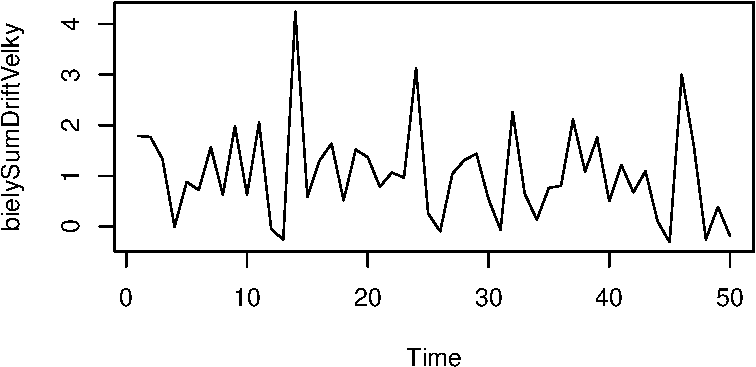
\includegraphics{prednaska3_NahodnaPrechadzkaStacionarita_files/figure-pdf/unnamed-chunk-11-3.pdf}

\begin{Shaded}
\begin{Highlighting}[]
\FunctionTok{mean}\NormalTok{(bielySumDriftVelky)}
\end{Highlighting}
\end{Shaded}

\begin{verbatim}
[1] 1.038807
\end{verbatim}

\begin{Shaded}
\begin{Highlighting}[]
\FunctionTok{var}\NormalTok{(bielySumDriftVelky)}
\end{Highlighting}
\end{Shaded}

\begin{verbatim}
[1] 0.8667145
\end{verbatim}

\begin{Shaded}
\begin{Highlighting}[]
\FunctionTok{sqrt}\NormalTok{(}\FunctionTok{var}\NormalTok{(bielySumDriftVelky))}
\end{Highlighting}
\end{Shaded}

\begin{verbatim}
[1] 0.930975
\end{verbatim}

\begin{Shaded}
\begin{Highlighting}[]
\FunctionTok{arima}\NormalTok{(bielySumDriftVelky, }\AttributeTok{order =} \FunctionTok{c}\NormalTok{(}\DecValTok{0}\NormalTok{, }\DecValTok{0}\NormalTok{, }\DecValTok{0}\NormalTok{))}
\end{Highlighting}
\end{Shaded}

\begin{verbatim}

Call:
arima(x = bielySumDriftVelky, order = c(0, 0, 0))

Coefficients:
      intercept
         1.0388
s.e.     0.1303

sigma^2 estimated as 0.8494:  log likelihood = -66.87,  aic = 137.73
\end{verbatim}

Tu už vidieť, že rozdiel prvých diferencií je biely šum s priemerom 1.

\bookmarksetup{startatroot}

\chapter*{Záver}\label{zuxe1ver}
\addcontentsline{toc}{chapter}{Záver}

\markboth{Záver}{Záver}

\bookmarksetup{startatroot}

\chapter*{References}\label{references}
\addcontentsline{toc}{chapter}{References}

\markboth{References}{References}

\phantomsection\label{refs}
\begin{CSLReferences}{0}{1}
\end{CSLReferences}




\end{document}
